\documentclass{amsart}
%\documentclass{article}
%\documentclass[final,onecolumn]{IEEEtran}

%\documentclass[pdflatex,sn-mathphys]{sn-jnl}
%\documentclass[final]{IEEEtran}

%\IEEEoverridecommandlockouts
% The preceding line is only needed to identify funding in the first footnote. If that is unneeded, please comment it out.
\usepackage{cite}
\usepackage{amsmath,amssymb,amsfonts}
\usepackage{faktor}
\usepackage{bm}% bold math
\usepackage{algorithmic}
\usepackage{graphicx}
\usepackage{textcomp}
\usepackage{xcolor}
\usepackage{rotating, booktabs}
\usepackage{wallpaper}
\usepackage{amsmath}
\usepackage{amsthm}
\usepackage{amsfonts}
\usepackage{amssymb}
\usepackage{graphicx}
\usepackage{float}
\usepackage{subfigure}
\usepackage{makecell}
%\usepackage{filecontents}
\usepackage{hyperref}
\usepackage{indentfirst}
\usepackage{comment}
\usepackage{mathrsfs}
\usepackage{tikz}
%\def\BibTeX{{\rm B\kern-.05em{\sc i\kern-.025em b}\kern-.08em
%		T\kern-.1667em\lower.7ex\hbox{E}\kern-.125emX}}

\makeatletter
\def\@setthanks{\vspace{-\baselineskip}\def\thanks##1{\@par##1\@addpunct.}\thankses}
\makeatother

\newtheorem{definitionenv}{Definition}
\newtheorem{lemmaenv}[definitionenv]{Lemma}
\newtheorem{theoremenv}[definitionenv]{Theorem}
\newtheorem{corollaryenv}[definitionenv]{Corollary}
\newtheorem{propositionenv}[definitionenv]{Proposition}
\newtheorem{conjectureenv}[definitionenv]{Conjecture}
\newtheorem{problemenv}[definitionenv]{Problem}
\newtheorem{remarkenv}[definitionenv]{Remark}
\newenvironment{remark}{\begin{remarkenv}\rm}{\end{remarkenv}}
%\newcommand{\br}{\begin{remark}}
\newcommand{\er}{\end{remark}}

\newtheorem{exampleenv}{Example}
\newtheorem{app-lemmaenv}[section]{Lemma}

\newenvironment{problem}{\begin{problemenv}\rm}{\end{problemenv}}
\newenvironment{definition}{\begin{definitionenv}\rm}{\end{definitionenv}}
\newenvironment{lemma}{\begin{lemmaenv}\rm}{\end{lemmaenv}}
\newenvironment{theorem}{\begin{theoremenv}\rm}{\end{theoremenv}}
\newenvironment{corollary}{\begin{corollaryenv}\rm}{\end{corollaryenv}}
\newenvironment{example}{\begin{exampleenv}\rm}{\end{exampleenv}}
\newenvironment{proposition}{\begin{propositionenv}\rm}{\end{propositionenv}}
\newenvironment{conjecture}{\begin{conjectureenv}\rm}{\end{conjectureenv}}
\newenvironment{app-lemma}{\begin{app-lemmaenv}\rm}{\end{app-lemmaenv}}

\theoremstyle{definition}

\newcommand{\cA}{{\mathcal A}}
\newcommand{\cB}{{\mathcal B}}
\newcommand{\cP}{{\mathcal P}}

\newcommand{\bmo}{{\bm 0}}
\newcommand{\bml}{{\bm 1}}

\newcommand{\bma}{{\bm a}}
\newcommand{\bmb}{{\bm b}}
\newcommand{\bmc}{{\bm c}}
\newcommand{\bmd}{{\bm d}}
\newcommand{\bmg}{{\bm g}}
\newcommand{\bmh}{{\bm h}}
\newcommand{\bmi}{{\bm i}}
\newcommand{\bmj}{{\bm j}}
\newcommand{\bmn}{{\bm n}}
\newcommand{\bmk}{{\bm k}}
\newcommand{\bme}{{\bm e}}
\newcommand{\bms}{{\bm s}}
\newcommand{\bmt}{{\bm t}}
\newcommand{\bmu}{{\bm u}}
\newcommand{\bmv}{{\bm v}}
\newcommand{\bmx}{{\bm x}}
\newcommand{\bmy}{{\bm y}}
\newcommand{\bmz}{{\bm z}}
\newcommand{\bmp}{{\bm p}}
\newcommand{\bmr}{{\bm r}}
%\newcommand{\bml}{{\bm \ell}}
\newcommand{\bmw}{{\bm w}}

\newcommand{\rmark}[1]{{\color{red} #1}}
\newcommand{\bmark}[1]{{\color{blue} #1}}
\newcommand{\dist}[2]
{\langle#1, #2\rangle}

\providecommand{\keywords}[1]
{
  \small	
  \textbf{\textit{Keywords---}} #1
}



\begin{document}

	
\title[]{An Error-Correction Model for Information Transmissions of Social Networks}
\author[]{Daqi (Reinhardt) Fang$^1$$^2$$^3$}\thanks{
\noindent
$^1$Hangzhou Yungu School, Hangzhou, China. \\
$^2$Intellisia Institute, Guangzhou, China. \\
$^3$Center for Complex Decision Analysis, Fudan University, Shanghai, China.\\
Email: Reinhardt114514@outlook.com}
\author[]{Pin-Chieh Tseng$^4$}\thanks{\noindent$^4$Institute of Communications Engineering and the Department of Applied Mathematics, National Yang Ming Chiao Tung University (NYCU), Hsinchu 30010, Taiwan.\\
Email: pichtseng@gmail.com.}

	
\maketitle

\begin{abstract}
We study the error-correction problem of the communication between two vertices in a social network. By applying the concepts of coding theory into the Social Network Analysis (SNA), we develop the code social network model, which can offer an efficient way to ensure the correctness of the message transmission within the social netwoks. The result of this study could apply in vary of social science studies.

\smallskip
\noindent \textbf{Keywords.} Coding Theory, SNA
\end{abstract}



\section{Introduction}


\subsection{Overview of Apply Coding Theory and SNA}

The application of coding theory to social network analysis has been a topic of great interest in recent years. Coding theory is a branch of mathematics that deals with the efficient transmission of information over noisy channels. It is used to design codes that can be used to encode and decode messages, allowing for reliable communication even in the presence of noise.

Regarding to SNA, it has used in the various algorithms to analysis networks such as pathfinding algorithms (e.g., Dijkstra’s Algorithm), community detection algorithms (e.g., Girvan-Newman Algorithm), link prediction algorithms (e.g., Katz index), and graph embedding algorithms (e.g., DeepWalk, see: Perozzi, Al-Rfou and Skiena \cite{PAS14}) Pathfinding algorithms (Foead et al. \cite{FGKHG21}) are used to find the shortest path between two nodes while community detection algorithms are used to identify groups of nodes that are more densely connected than others in a network (Lancichinetti and Fortunato \cite{LF09}) Link prediction algorithms (Lü and Zhou \cite{LZ11}) are used to predict future connections between nodes while graph embedding algorithms are used to represent networks in low-dimensional vector spaces for further analysis or visualization purposes. Some others worth-noticing algorithms including the Node2Vec (Grover and June 2017), which is an algorithm for learning low-dimensional representations of nodes in a graph, and it uses random walks to explore the graph structure and learn node embeddings that capture both local and global network properties (For example: Hu et al. \cite{HLLL20}) Graph Convolutional Networks (GCN) algorithm that can be used to learn representations of nodes in a graph, and it has been used for tasks such as node classification, link prediction, and community detection (Zhang et al. \cite{ZTXM19}) GraphSAGE is an inductive representation learning algorithm (Hamilton, Ying and Leskovec \cite{HYL17}) for graphs can be used for tasks such as node classification, link prediction, and community detection. 

SNA has been used to study a variety of topics, such as the spread of disease, the diffusion of innovations, and the formation of social movements. Despite its widespread use in many areas, there is still a lack of research and modeling of information transmission within social networks in SNA.



\subsection{Limitations of Information Transmission of the SNA}

Information transmission is an important process in social networks because it allows for the spread of ideas and knowledge among individuals. This process can be studied through various methods such as surveys, interviews, or experiments. However, these methods are often limited in their ability to capture the complexity of information transmission within social networks. As a result, there is a need for more research into how information flows through social networks and how it affects behavior and outcomes.

The first limitation of SNA is that it relies on data from existing networks and hard to simulation. This means that it hard to simulate or capture information about new connections or changes within an existing connections of social network. Additionally, current studies about SNA do not consider the size and transmitted bound in which information is transmitted or received systematically by mathematical method.

A second limitation of SNA is that it does not capture the content of information transmission. While currently SNA can provide insight into how information spreads within a network, it cannot provide insight into what type of information is being shared or how it is being interpreted by different individuals within the network, or how the nodes within a social network made the error and error-correcting. This can lead to inaccurate conclusions about how information spreads within a network and how it affects behavior within the network. For example, what political scientists consider to be a considerable degree of the failure of Zhao Ziyang's faction during the Tiananmen crisis in 1989 (Fewsmith \cite{Few09}; Ziyang \cite{Ziy09}) appears to us to be, to some extent, information transmission errors within his factional network.

Currently, there has two ways to study information transmission within social networks. First one is through Agent-Based Modeling (ABM), which is a type of computer simulation that uses agents—individuals or entities—to represent different actors in a system. These agents interact with each other according to certain rules that are programmed into the model (For example: Frias-Martinez, Williamson and Frias-Martinez \cite{FWF11}; Lane \cite{Lan18}; Li et at. \cite{LYJWL21}) Another way to study information transmission within social networks is through network analysis tools such as graph theory or Exponential Random Graph Models (ERGMs), it provides insights into the structure of a network by analyzing its nodes (individuals) and edges (relationships between individuals).

However, research about information transmission within social networks is still lacking in terms of mathematical algorithms. Algorithms are the backbone of any meaningful SNA, as they are responsible for organizing and managing the information within the social networks. 

\subsection{Structure}
Section 2 is a quick review for some basic concept.
In section 3, we will define what is Coding Social Network (CSN), by explaining background parameters, introducing how to encode the most basic simple social network. Then we will classifying the different types of simple CSN
In section 4, we will explain how to perform error detection and correction for complex social networks (usually, a complex social network is composed of multiple simple social networks). And we will encode a ``prefect covering social network" and give examples.
In section 5, we will calculate the upper bound of CSN.



\subsection{Academic Contribution of Our Study}

In the context of SNA, coding theory can be used to encode the message and do error-correcting. For example, it can be used to reduce the amount of noise in a network by encoding messages using an error-correcting code. This allows for more accurate to see transmission of information between nodes in a network, as well as could reviewing and reducing the amount of information that needs to be transmitted within social networks. Moreover, we could find a ``perfect-network" by our construction.

By applying coding theory to SNA, researchers can identify patterns and relationships within social networks that would otherwise be difficult to detect. This has led to a better understanding of how social networks operate and how they influence individual behavior and decision-making. In political science, SNA could use into studies about the formation of interest groups, the spread of political ideologies, and the dynamics of political campaigns. In sociology, SNA could use into study social stratification, the diffusion of cultural norms, and the formation of social movements. Overall, the application of coding theory in SNA has provided valuable insights into the workings of complex social systems and has helped researchers develop new theories about human behavior and interaction.

\section{Preliminaries}
In this section, we give a quick review for some basic concepts of error-correction codes. For more details, we recommend readers the book \cite{MS77}.

Let $\mathcal{P}_{n}$ be the collection of all vectors in $F_{q}^{n}$, where $F_{q}$ is a finite field with $q$ elements. A code $C$ of length $n$ is defined as a subset of $\mathcal{P}_{n}$. The elements of $C$ are called codewords. Moreover, for $a = (a_{1}, \dots, a_{n})$, $b(b_{1}, \dots, b_{n}) \in \mathcal{P}_{n}$, we can define their Hamming distance as follows:
\[
d_{H}(a, b) = \lvert \{i : a_{i} \neq b_{i}\} \rvert.
\]
The minimum distance $d$ of a code $C$ is described as the minimum Hamming distance between codewords in $C$. Moreover, the weight of a codeword $a$ is defined as 
\[
{\rm wt}(a) = d(a, \overline{0}),
\]
where $\overline{0}$ is the zero vector. The minimum distance is high related to the ability of error detection and error correction. A code with minimum distance $d$ can detect $d-1$ errors and correct $\lfloor \frac{d-1}{2} \rfloor$ errors. 

For general $C$, to check if a codeword $a$ contains an error, we need to check whether $a \in C$ or not. It may cost lots of time when $q$ is large. In here, we also introduce a special code structure, which provide a convenient way to deal with this problem, called linear code. A linear code $C$ is defined as a $k$-dimensional subspace of $F_{q}^{n}$. Moreover, a linear code can be generated by an $n \times k$ matrix $M$ such that $C = {\rm Im}(M)$. In this case, $M$ is called the generated matrix of $C$. The encoding process $E$ for message $m$ can be defined as follows:
\[
E(m) = M m.
\]
For the matrix $M$, there exists an $(n-k)\times n$ matrix $N$ with rank $n-k$ satisfying $NM = 0$. $N$ is called the parity check matrix and for $a \in F_{q}^{n}$, $a \in C$ if and only if $N a = 0$. Moreover, we denote $C$ by the parameter $[n, k, d]_{q}$, where $n$ is the length of $C$, $k$ is the dimension of $C$ as a subspace and $d$ is the minimum distance.

\begin{example}
    We define $C = [7, 4, 3]_{2}$ by the generated matrix
\[
    M = 
    \begin{pmatrix}
        1 & 0 & 0 & 0\\
        0 & 1 & 0 & 0\\
        0 & 0 & 1 & 0\\
        0 & 0 & 0 & 1\\
        0 & 1 & 1 & 1\\
        1 & 0 & 1 & 1\\
        1 & 1 & 0 & 1\\
    \end{pmatrix}.
\]
Then, the parity check matrix can be taken as
\[
    N = 
    \begin{pmatrix}
        0 & 0 & 0 & 1 & 1 & 1 & 1\\
        0 & 1 & 1 & 0 & 0 & 1 & 1\\
        1 & 0 & 1 & 0 & 1 & 0 & 1\\
    \end{pmatrix}.
\]
\end{example}

\section{Code social network}

\subsection{From social network to code social network}
\begin{figure}[b]
    \centering
    \begin{tikzpicture}
    [scale=.8]
    \node (n6) at (1,10) {6};
    \node (n4) at (4,8)  {4};
    \node (n5) at (8,9)  {5};
    \node (n1) at (11,8) {1};
    \node (n2) at (9,6)  {2};
    \node (n3) at (5,5)  {3};

    \foreach \from/\to in   {n6/n4,n4/n5,n5/n1,n1/n2,n2/n5,n2/n3,n3/n4}
    \draw (\from) -- (\to);

    \end{tikzpicture}
    \caption{$S = (V, D)$ with $V = \{1, 2, 3, 4, 5, 6\}$ and $D = \{(1, 2), (1, 5), (2, 3), (2, 5), (3, 4), (4, 5), (4, 6)\}$.}
    \label{fig:ex_S}
\end{figure}

Now, we define $S = (V, D)$ to be a social network with vertex set $V$ and edge set $D$. Note that in the following, we use the word ``vertex" to replace ``node" in social network analysis and regard a social network as a graph. For our description, we give an example in Figure \ref{fig:ex_S}. Then, we define the code social network(CSN) $\hat{S} = (S, C, f)$ as a weighted network which has the same vertex set and edge set as $S$ together with a code $C \subset F_{q}$. Let $a = (a_{1}, \dots, a_{n}) \in C$. An error occurring on $a_{i}$ is assumed as a map sending $a_{i}$ to an element of $F_{q} \setminus a_{i}$ randomly. For $(\alpha, \beta) \in D$, we denote the probability that an error occurs on $a_{i}$ when $\alpha$ sends $a$ to $\beta$ by $p_{(\alpha, \beta)}(a_{i})$. To simplify our model, we assume that the probability $p_{(\alpha, \beta)}(a_{i})$ is independent on the component $i$ and the codeword $a$. Moreover, we denote $p_{(\alpha, \beta)}(a_{i})$ as $p_{(\alpha, \beta)}$. Then, we weight the edge $(\alpha, \beta)$ by the weight function $f$ defined by $f(\alpha, \beta) = p_{(\alpha, \beta)}$. 

\begin{definition}
    Let $\alpha, \beta \in V$ and $P_{(\alpha, \beta)} = (\alpha = \gamma_{0}, \gamma_{1}, \dots, \gamma_{l} = \beta)$ be a path from $\alpha$ to $\beta$ on the weighted network $\hat{S}$. Now, $\alpha$ sends a codeword $a$ along the path ${\rm Path}_{(\alpha, \beta)}$ to $\beta$ and $\beta$ receives the codeword $a'$. Let $E_{(\alpha, \beta)}$ be the expectation value of the Hamming distance $d_{H}(a, a')$. Then, we define the follows.
    \begin{enumerate}
        \item 
        $P_{(\alpha, \beta)}$ is said to be efficient if $ E_{P_{(\alpha, \beta)}} \leq \lfloor \frac{d-1}{2} \rfloor$,
        \item
        $P_{(\alpha, \beta)}$ is said to be semi-efficient if $E_{P_{(\alpha, \beta)}} \leq d-1$,
        \item
        $P_{(\alpha, \beta)}$ is said to be inefficient if $E_{P_{(\alpha, \beta)}} > d-1$.
    \end{enumerate}
\end{definition}

\begin{remark}
    Under our definition and assumption, for two paths $P_{(\alpha, \beta)}, P'_{(\alpha, \beta)}$ with $P_{(\alpha, \beta)}$ has a longer length, we do not have $E_{P(\alpha, \beta)} \geq E_{P'(\alpha, \beta)}$.
\end{remark}


\begin{definition}
    Let $\hat{S} = (S, C, f)$ be a CSN. We define the follows.
    \begin{enumerate}
        \item 
        $\hat{S}$ is said to be efficient if for each $\alpha, \beta \in V$, the shortest path from $\alpha$ to $\beta$ is efficient,
        \item
        $\hat{S}$ is said to be semi-efficient if for each $\alpha, \beta \in V$,  the shortest path from $\alpha$ to $\beta$ is semi-efficient,
        \item
        $\hat{S}$ is said to be inefficient if $\hat{S}$ is not semi-efficient,
        \item
        The critical value $\mathscr{C}(\hat{S})$ of $\hat{S}$ as
        \[
        \mathscr{C}(\hat{S}) = {\rm max}\{l(\alpha, \beta) \mid (\alpha, \beta) \in D\},
        \]
        where $l(\alpha, \beta)$ is denoted by the length of the shortest path from $\alpha$ to $\beta$.
    \end{enumerate}
\end{definition}

\begin{lemma}
    \label{lem:CSN_bin}
    Suppose $f(\alpha, \beta) = p$ is constant for $(\alpha, \beta) \in D$, $C \subset F_{2}^{n}$. Then, 
    \begin{enumerate}
        \item 
        $\hat{S}$ is efficient if and only if
        \[
        n \sum_{k = 0}^{\left\lfloor \frac{l}{2} \right\rfloor} \binom{l}{2k+1} p^{2k+1} (1-p)^{l-2k-1}  \leq \left\lfloor \frac{d-1}{2} \right\rfloor
        \]
        for $1 \leq l \leq \mathscr{C}(\hat{S})$,
        \item
        $\hat{S}$ is semi-efficient if and only if
        \[
        n \sum_{k = 0}^{\left\lfloor \frac{l}{2} \right\rfloor} \binom{l}{2k+1} p^{2k+1} (1-p)^{l-2k-1} \leq d-1
        \]
        for $1 \leq l \leq \mathscr{C}(\hat{S})$,
        \item
        $\hat{S}$ is inefficient if and only if
        \[
        n \sum_{k = 0}^{\left\lfloor \frac{l}{2} \right\rfloor} \binom{l}{2k+1} p^{2k+1} (1-p)^{l-2k-1} > d-1
        \]
        for $1 \leq l \leq \mathscr{C}(\hat{S})$.
    \end{enumerate}
\end{lemma}

\begin{proof}
Since $C \subset F_{2}^{n}$, for a codeword $a = (a_{1}, \dots, a_{n}) \in C$, two errors occur on $a_{i}$ implies $a_{i}$ is not changed. Thus, we only need to consider that for each component, there are only odd edges which cause error. Then, the expectation value of the number of errors which may change the codeword within path of length $l$ can be calculated as
\[
n \sum_{k = 0}^{\left\lfloor \frac{l}{2} \right\rfloor} \binom{l}{2k+1} p^{2k+1} (1-p)^{l-2k-1}.
\]
\end{proof}

\begin{lemma}
    \label{lem:CSN_nonbin}
    Suppose $f(\alpha, \beta) = p$ is constant for $(\alpha, \beta) \in D$ and $C \subset F_{q}^{n}$. We define the sequences $\{A_{i}\}$, $\{B_{i}\}$ by the recurrence relation
    \[
    A_{1} = p, \quad B_{1} = 1-p,
    \]
    \[
    A_{j} = A_{j-1} p \frac{q-2}{q-1} + B_{j-1} p, \quad B_{j} = A_{j-1} p \frac{1}{q-1} + B_{j-1} (1-p).
    \]
    Then, 
    \begin{enumerate}
        \item 
        $\hat{S}$ is efficient if and only if $nA_{l} \leq \lfloor \frac{d-1}{2} \rfloor$ for $1 \leq l \leq \mathscr{C}(\hat{S})$.
        \item
        $\hat{S}$ is semi-efficient if and only if $nA_{l} \leq d-1$ for $1 \leq l \leq \mathscr{C}(\hat{S})$.
    \end{enumerate}
\end{lemma}

\begin{proof}
    According to the above definitions, $A_{i}$ represents the probability that by comparing with the original codeword, an error occurs on one component of the message after passing $i$ edges within a social network. Then, we have the result.
\end{proof}

\subsection{Transmission path on efficient CSN}
\label{sec:trans_path}

Let $\hat{S} = (S, C, f)$ be an efficient CSN. In this part, we give a convenient method to figure out the transmission path from $\alpha$ to $\beta$ by labeling each vertex a codeword in $F_{q}^{N}$ for some $N$ is sufficient large. First, we start with the definition.

\begin{definition}
    Let $\hat{S} = (S, C, f)$ be an efficient CSN. If there is a spanning tree $T = (V, D')$ such that $\hat{T} = (T, C, f')$ with
    \[
    f(\alpha, \beta) = f'(\alpha, \beta) \text{ for } (\alpha, \beta) \in D'
    \]
    is efficient, $\hat{S}$ is called super-efficient.
\end{definition}

For a super-efficient CSN $\hat{S}$ together with an efficient $\hat{T}$, our goal is to label each vertex in $V$ by the function $\phi$, which is an injective map from $V$ to $F_{q}^{N}$ such that for $\alpha, \beta \in V$, the path from $\alpha$ to $\beta$ in $T$ can be determined by comparing $\phi(a)$ with $\phi(b))$. Here, we present the rules for defining $\phi$.
\begin{enumerate}
    \item 
    If $\gamma$ is the root of $T$, $\phi(\gamma)$ is the zero vector.
    \item
    Let $(\alpha, \beta) \in D'$ with $\alpha$ is labeled and $\beta$ is unlabeled. Let $\phi(\alpha) = (a_{1}, \dots, a_{N})$ and $k = {\rm max}\{i : a_{i} \neq 0\}$. If there is $b_{k+1}$ such that the codeword $b = (a_{1}, \dots, a_{k}, b_{k+1}, 0, \dots, 0)$ is not used, let $\phi(\beta) = b$. Otherwise, we label $\beta$ by the vector $(a_{1}, \dots, a_{k}, 0, 1, 0 \dots, 0)$.
\end{enumerate}

Under this labeling, if $\alpha$ wants to send a message to $\beta$ with knowing $\phi(\beta)$, a good transmission path can be found as follows.
\begin{enumerate}
    \item 
    If ${\rm wt}(\phi(\alpha)) \geq {\rm wt}(\phi(\beta))$, $a$ should send the message to the vertex which is labeled as the codeword obtained by changing the last non-zero term in $\phi(\alpha)$ to $0$.
    \item
    If ${\rm wt}(\phi(\alpha)) < {\rm wt}(\phi(\beta))$, $\beta$ should receive the message from the vertex which is labeled as the codeword obtained by changing the last non-zero term in $\phi(\beta)$ to $0$.
\end{enumerate}

\begin{example}
\label{exp:path_tree}
    Let $S = (V, D)$ with $V = \{1, 2, 3, 4, 5, 6\}$ and $D = \{(1, 2)$, $(1, 5)$, $(2, 3), (2, 5), (3, 4), (4, 5), (4, 6)\}$. Let $C \subset F_{2}^{n}$ be a code with minimum distance $d \geq \frac{n}{50} + 1$ and $n = 10$. Let $f(a, b) = p = \frac{1}{100}$ for all $(a, b) \in D$. We define $\hat{S} = (S, C, f)$ and obvious that $\mathscr{C}(\hat{S}) = 3$. Then, by applying Lemma \ref{lem:CSN_bin}, we can check $np = \frac{n}{100}$, $2n p(1-p) = \frac{99n}{5000}$ and
    \begin{align*}
    n \sum_{k = 0}^{\left\lfloor \frac{\mathscr{C}(\hat{S})}{2} \right\rfloor} \binom{\mathscr{C}(\hat{S})}{2k+1} p^{2k+1} (1-p)^{\mathscr{C}(\hat{S})-2k-1} &= n \left(3 p (1-p)^{2} + p^{3}\right)\\
    &= \frac{9802 n}{10^{6}}.
    \end{align*}
    Thus, $\hat{S}$ is efficient. Let $T = (V, D')$ with $D' = \{(6, 4), (4, 3), (4, 5), (5, 2), (5, 1)\}$. We can calculate that $\hat{S}$ is super-efficient together with the spanning tree $T$. We define $\phi$ as a map from $V$ to $F_{2}^{5}$ by 
    \begin{align*}
        &\phi(6) = (0, 0, 0, 0, 0), \quad \phi(4) = (1, 0, 0, 0, 0),\\
        &\phi(3) = (1, 1, 0, 0, 0), \quad \phi(5) = (1, 0, 1, 0, 0),\\
        &\phi(2) = (1, 0, 1, 1, 0), \quad \phi(1) = (1, 0, 1, 0, 1),
    \end{align*}
    and 
    \begin{align*}
    {\rm Im}(\phi) = \{&(0, 0, 0, 0, 0), (1, 0, 0, 0, 0), (1, 1, 0, 0, 0),\\
    &(1, 0, 1, 0, 0), (1, 0, 1, 1, 0), (1, 0, 1, 0, 1)\}.
    \end{align*}
    When vertex $6$ wants to send a message to vertex $1$, ${\rm wt}(\phi(6)) = 0 < 3 = {\rm wt}(\phi(1))$ implies that we should compare $\phi(6)$ with $\phi(1)$ and figure out what $j$ is. By observing $j = 1$, vertex $6$ should send the message to vertex $4$ which is labeled by $(1, 0, 0, 0, 0)$. By repeating this process, vertex $4$ should send the message receiving from vertex $6$ to vertex $5$ with the label $(1, 0, 1, 0, 0)$. Then, vertex $5$ sends the message to vertex $1$.
    \begin{align*}
    &\phi(6) = (0, 0, 0, 0, 0) \rightarrow \phi(4) = (1, 0, 0, 0, 0) \rightarrow \\
    &\phi(5) = (1, 0, 1, 0, 0) \rightarrow \phi(1) = (1, 0, 1, 0, 1).
    \end{align*}
    Now, we consider the case that vertex $3$ wants to send a message to vertex $2$. ${\rm wt}(\phi(3)) = 2 < 3 = {\rm wt}(\phi(2))$ and the $2$th component of $\phi(3)$ is $1$ but $\phi(2)$ contains $0$ in the same position. By our rule, vertex $3$ should send the message to a vertex, which is labeled by $(1, 0, 0, 0, 0)$. That is vertex $4$. Then, vertex $4$ should compare $\phi(4)$ with $\phi(2)$ and figure out the label by changing the third component of $\phi(4)$ to $1$. Then, vertex $4$ should send the message to the vertex $5$. Then, vertex $5$ sends the message to vertex $2$.
    \begin{align*}
    &\phi(3) = (1, 1, 0, 0, 0) \rightarrow \phi(4) = (1, 0, 0, 0, 0) \rightarrow \\
    &\phi(5) = (1, 0, 1, 0, 0) \rightarrow \phi(2) = (1, 0, 1, 1, 0).
    \end{align*}
\end{example}

\begin{remark}
Each vertex in an efficient CSN only needs to keep the code ${\rm Im}(\phi)$ and compare the label of itself with the terminal vertex to find a path, which is good enough in the sense of error-correction (but not necessary to be the shortest path), instead of using the traditional Dijkstra Algorithm to figure out and save every shortest paths.
\end{remark}

\begin{remark}
    For efficient CSNs, we can classify them into the following three classes. 
    \begin{enumerate}
        \item 
        If $S$ is a tree, we say that $\hat{S}$ is in type $A$.
        \item
        If $S$ is dense but not a tree, we say $\hat{S}$ is in type $B$.
        \item
        If $S$ is a complete graph, we say $\hat{S}$ is in type $C$.
    \end{enumerate}
    Readers might refer Figure \ref{fig:type} as an example. Clearly, for type $A$, our method mentioned before always use the shortest path. For type $C$, we can label the vertices by codewords in a simplex code. Under this method, we can identify whether $S$ is a complete graph or not by observing the codewords so that in the case of type $C$, we can use the shortest path to complete our transmission.
\end{remark}

\begin{figure}
    
    \centering
    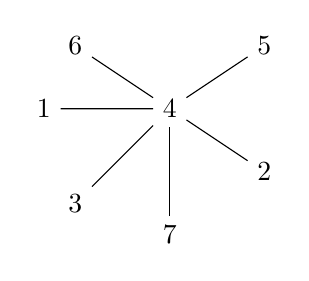
\begin{tikzpicture}
    [scale=.4]
    \node (n6) at (1,10) {6};
    \node (n4) at (4,8)  {4};
    \node (n5) at (7,10)  {5};
    \node (n1) at (0,8) {1};
    \node (n2) at (7,6)  {2};
    \node (n3) at (1,5)  {3};
    \node (n7) at (4,4)  {7};

    \foreach \from/\to in   {n6/n4,n4/n5,n4/n1,n4/n2,n4/n3,n7/n4}
    \draw (\from) -- (\to);

    \end{tikzpicture}
    \quad \quad
    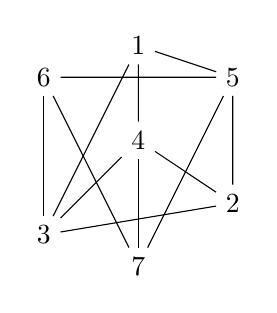
\begin{tikzpicture}
    [scale=.4]
    \node (n6) at (1,10) {6};
    \node (n4) at (4,8)  {4};
    \node (n5) at (7,10)  {5};
    \node (n1) at (4,11) {1};
    \node (n2) at (7,6)  {2};
    \node (n3) at (1,5)  {3};
    \node (n7) at (4,4)  {7};

    \foreach \from/\to in   {n2/n3,n6/n3,n1/n3,n6/n7,n1/n5,n6/n5,n5/n2,n5/n7,n4/n1,n4/n2,n4/n3,n7/n4}
    \draw (\from) -- (\to);

    \end{tikzpicture}
    \quad \quad
    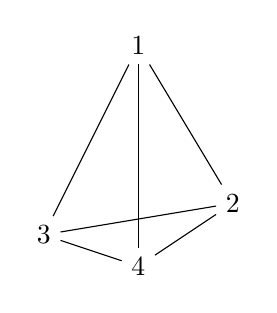
\begin{tikzpicture}
    [scale=.4]
    \node (n1) at (4,11) {1};
    \node (n2) at (7,6)  {2};
    \node (n3) at (1,5)  {3};
    \node (n4) at (4,4)  {4};

    \foreach \from/\to in   {n1/n2,n1/n3,n1/n4,n2/n3,n2/n4,n3/n4}
    \draw (\from) -- (\to);

    \end{tikzpicture}
    \caption{The graph in the left is type $A$. The middle one is type $B$. The graph in the right is type $C$.}
    \label{fig:type}
\end{figure}

\begin{remark}
    The social network can be seen in many different forms in our society. For example, the political factionalism of the USSR and China is a prime example of a social network. This type of network is characterized by composing of multiple political etlites that are connected through a complex web of alliances and co-interests. Additionally, interest groups lobby-networks in the United States are another example of a non-digraph social network. These networks are composed of various interest groups that are attempting to influence policy decisions through lobbying efforts. Finally, kinship networks within ancient China can also be considered as a type of non-digraph and muti-centralized complex social network (a complex version of our type B in Figure 2) since they involve multiple nodes who are connected through a key kinship node, and this character also made contributions of state building in imperial China (Wang \cite{Wan22}). 
 

\end{remark}




\section{Error detection and correction in Complex CSN}

In this section, we start to apply our model to more complex cases.

\subsection{Covering by super-efficient CSNs}

For a non-efficient CSN $\hat{S}=(S, C, f)$ and vertices $\alpha, \beta$, there might not exist an efficient path from $\alpha$ to $\beta$. To deal with this situation, our approach is to cover each vertices in $\hat{S}$ by super-efficient CSNs $\{\hat{S}_{i}=(S_{i}, C, f)\}$ with each $S_{i} = (V_{i}, D_{i})$ is an induced subgraph of $S$. Furthermore, to allow the transmission between different $\hat{S}_{i}$, we need to use a ``reachable" covering.

\begin{definition}
    Let $N = \{\hat{S}_{i}\}$ be a collection of CSNs.
    \begin{enumerate}
        \item 
        $N$ is said to be a covering of $\hat{S}$ if each $S_{i}$ is an induced subgraph of $S$ and $\bigcup_{i} V_{i} = V$.
        \item
        A covering $N$ of $\hat{S}$ is said to be reachable if for every subset $A$ of $\mathcal{P} = \{1, \dots, \lvert N \rvert\}$, 
        \[
        \bigcup_{i \in A} V_{i} \cap \bigcup_{i \in \mathcal{P} \setminus A} V_{i} \neq \emptyset.
        \]
    \end{enumerate}
\end{definition}

\begin{definition}
    We say that $N = \{\hat{S}_{i}\}$ is an efficient covering of $\hat{S}$ if 
    \begin{enumerate}
        \item 
        $\hat{S}_{i}$ is super-efficient for each $i$,
        \item
        $N$ is a covering of $\hat{S}$, and
        \item
        $N$ is reachable.
    \end{enumerate}
\end{definition}

Under this definition, every efficient covering offers a transmission path for a pair of vertices in $\hat{S}$. Let $\alpha, \beta$ be two vertices. Then, there exist $i, j$ such that $\alpha$ is a vertex of $\hat{S}_{i}$ and $\beta$ is a vertex of $\hat{S}_{j}$. Because of the reachable property, there exist a sequence of super-efficient CSNs $\{\hat{S}_{a_{k}}\}_{k = 1}^{m}$ for some integer $m$ such that 
\begin{enumerate}
    \item $\hat{S}_{a_{0}} = \hat{S}_{i}$,
    \item $\hat{S}_{a_{m}} = \hat{S}_{j}$,
    \item $V_{a_{k}} \cap V_{a_{k+1}} \neq \emptyset$ for all $k$.
\end{enumerate}
Now, the transmission process from $\alpha$ to $\beta$ follows the steps:
\begin{enumerate}
    \item $\alpha$ sends a message to a vertex $\alpha_{1}$ in $V_{a_{0}} \cap V_{a_{1}}$. Then, $\alpha_{1}$ dose once error-correction process.
    \item
    For each $1 
    \leq k \leq m-1$, $\alpha_{k}$ sends a message to a vertex $\alpha_{k+1}$ in $V_{a_{k}} \cap V_{a_{k+1}}$. Then, $\alpha_{k+1}$ dose once error-correction process.
    \item $\alpha_{m}$ sends the message to $\beta$. Then, $\beta$ dose once error-correction and decoding process to obtain the information.
\end{enumerate}

To simplify our model, we suppose $f$ is a constant map. Using the formulas described in Lemma \ref{lem:CSN_bin} and Lemma \ref{lem:CSN_nonbin}, we can estimate an integer $r$ such that every path with length less or equal to $r$ is efficient. For a vertex $\alpha$ and an integer $k$, we define $B_{k}(\alpha)$ as the induced subgraph with vertex set
\[
\{\beta \in V : d_{G}(\alpha, \beta) \leq k\},
\]
where $d_{G}(\alpha, \beta)$ denotes the length of the shortest path from $\alpha$ to $\beta$. Under our assumption, the CSN $(B_{\lfloor\frac{r}{2}\rfloor}(\alpha), C, f)$ is super-efficient. 



\begin{definition}
    A subset $M_{r} = \{\alpha_{i}\} \subset V$ is said to be a covering set of $\hat{S}$ if $\{(B_{r}(\alpha_{i}), C, f)\}$ forms an efficient covering of $\hat{S}$. Moreover, the maximum integer $r$ such that the covering set $M_{r}$ of $\hat{S}$ exists is called the radius of $\hat{S}$.
\end{definition}

\begin{remark}
    Finding the smallest covering set of $\hat{S}$ is high related to the problem of minimum $k$-path vertex cover, which has been studied in \cite{BKKS11}, \cite{LZX16}, and \cite{YSM16}.
\end{remark}

Every covering set represents a transmission method for every two vertices of $\hat{S}$. Moreover, the size of a covering set implies the maximum times of error-correction process should be applied during the transmission.

\subsection{Perfect covering}

In this part, we consider CSNs with a great structure, which is called perfect covering.

\begin{definition}
Let $\hat{S}$ be a CSN.
\begin{enumerate}
    \item 
    An efficient covering $N$ of $\hat{S}$ is said to be perfect if for every $\hat{S}_{i}$, $\hat{S}_{j} \in N$, $V_{i} \cap V_{j} \neq \emptyset$.
    \item 
    $\hat{S}$ is called perfect if there exists a perfect covering.
\end{enumerate}
\end{definition}
With the given definition, we observe the simple result.
\begin{lemma}
    Every transmission process between two vertices in a perfect CSN only need to do the error-correction process twice.
\end{lemma}

\begin{figure}
    
    \centering
    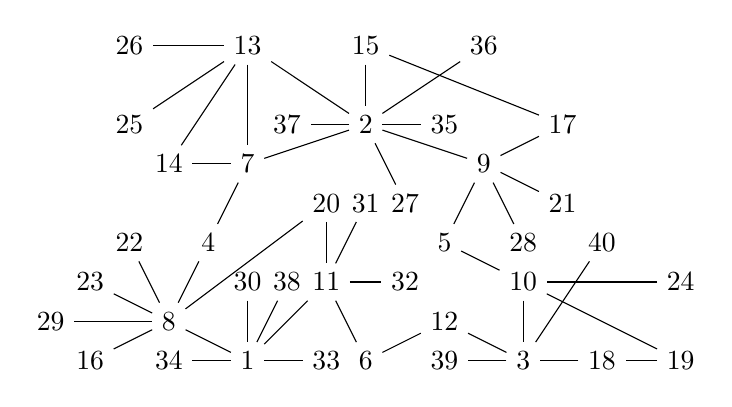
\begin{tikzpicture}
    [scale=.5]
    \node (n1) at (1,2) {1};
    \node (n2) at (4,8)  {2};
    \node (n3) at (8,2)  {3};
    \node (n4) at (0,5)  {4};
    \node (n7) at (1,7)  {7};
    \node (n8) at (-1,3)  {8};
    \node (n5) at (6,5)  {5};
    \node (n9) at (7,7)  {9};
    \node (n10) at (8,4)  {10};
    \node (n6) at (4,2)  {6};
    \node (n11) at (3,4)  {11};
    \node (n12) at (6,3)  {12};
    \node (n13) at (1,10)  {13};
    \node (n14) at (-1,7)  {14};
    \node (n15) at (4,10)  {15};
    \node (n16) at (-3,2)  {16};
    \node (n17) at (9,8)  {17};
    \node (n18) at (10,2)  {18};
    \node (n19) at (12,2)  {19};
    \node (n20) at (3,6)  {20};
    \node (n21) at (9,6)  {21};
    \node (n22) at (-2,5)  {22};
    \node (n23) at (-3,4)  {23};
    \node (n24) at (12,4)  {24};
    \node (n25) at (-2,8)  {25};
    \node (n26) at (-2,10)  {26};
    \node (n27) at (5,6)  {27};
    \node (n28) at (8,5)  {28};
    \node (n29) at (-4,3)  {29};
    \node (n30) at (1,4)  {30};
    \node (n31) at (4,6)  {31};
    \node (n32) at (5,4)  {32};
    \node (n33) at (3,2)  {33};
    \node (n34) at (-1,2)  {34};
    \node (n35) at (6,8)  {35};
    \node (n36) at (7,10)  {36};
    \node (n37) at (2,8)  {37};
    \node (n38) at (2,4)  {38};
    \node (n39) at (6,2)  {39};
    \node (n40) at (10,5)  {40};

    \foreach \from/\to in   {n1/n8,n8/n4,n4/n7,n7/n2,n2/n9,n9/n5,n5/n10,n10/n3,n1/n11,n11/n6,n6/n12,n12/n3,n13/n7,n14/n7,n15/n2,n16/n8,n17/n9,n18/n3,n19/n18,n10/n19,n20/n11,n9/n21,n22/n8,n20/n8,n15/n17,n13/n14,n23/n8,n24/n10,n13/n2,n25/n13,n26/n13,n2/n27,n9/n28,n29/n8,n30/n1,n11/n31,n11/n32,n1/n33,n1/n34,n2/n35,n2/n36,n2/n37,n1/n38,n3/n39,n3/n40}
    \draw (\from) -- (\to);

    \end{tikzpicture}
    \caption{The graph $S$ constructed by using the vertex set $M = \{1, 2, 3\}$ of a simplex in $\mathbb{R}^{2}$ and $k = 2$.}
    \label{fig:ex3}
\end{figure}


Next, we present a convenient approach to construct a perfect CSN. Let $k$ be given and $M$ be a collection of vertices of a simplex in $\mathbb{R}^{n}$. Now, for every $a, b \in M$, we place a vertex $e$ and two sequences of vertices $\{a_{i}\}_{i = 1}^{k-1}, \{b_{i}\}_{i = 1}^{k-1}$. Then, we add edges $(a, a_{1}), (b, b_{1}), (a_{k-1}, e), (b_{k-1}, e), (a_{i}, a_{i+1}),$ and $(b_{i}, b_{i+1})$ for each $i = 1, \dots k-2$. Moreover, around each $a \in M$, we might add vertices and edges such that all of those vertices can be connected to $a$ by a path with length less than $k$. Under this construction, we obtain a connected graph $S$. By choosing proper $C$ and $f$ such that every path with length less or equal to $2k$ is efficient, we construct a CSN $\hat{S} = (S, C, f)$ with a covering set $M_{k} = M$.

\begin{example}
    Let $M = \{1, 2, 3\}$ be the vertex set of of a simplex in $\mathbb{R}^{2}$ and $k$ = 2. Applying the method we mention before, we construct the CSN $\hat{S}$ by the graph $S$ described in Figure \ref{fig:ex3} and some proper $C$, $f$. Under $\hat{S}$, if vertex $1$ wants to send a message to vertex $17$, vertex $1$ should encode the message by the code $C$ and send the message along an efficient path to vertex $4$ first. Then, vertex $4$ dose once error-correction process. Next, vertex $4$ sends the message to vertex $17$. Final, vertex $17$ implement the error-correction and decoding process to obtain the message.
\end{example}

\begin{example}

Although the perfect social network is difficult to find in real society ,inefficient social networks which have inefficient information transmission examples are vasely. Inefficient information transmission can lead to information asymmetry, which occurs when one party has access to more or better information than the other, when one party has an informational advantage, they may be able to exploit this advantage to gain a better outcome for themselves at the expense of the other party (For example: \cite{Gun15}, \cite{GWZ18}, \cite{RW17}) The inefficient decision-making, especially in the public policy, is also a significant outcome of inefficient information transmission within the social network (For example: \cite{LM20}, \cite{WM20}, \cite{ZQVEW19})   
  
Our aim in this example is to showcase the inefficiency of Hu Jintao's leadership through an example of Chinese elite politics. According to a multitude of elites, his leadership has been widely criticized for being ineffective. Keller \cite{kel16} has conducted remarkable research on Chinese political elites, and we will utilize her work by coding and applying our algorithm based on the Chinese political elite network of 2012 drawn by Keller. This will enable us to demonstrate the inefficiency of the social network during the Hu Jintao era.

If Liu Yuan wants to send a message to Hu Chunhua, the shortest path is
\[
\text{Liu Yuan} \rightarrow \text{Xi Jinping} \rightarrow \text{Li Zhanshu} \rightarrow \text{Hu Jintao} \rightarrow \text{Hu Chunhua}.
\]

Take $p = 0.75$, we can calculate
\[
n \sum_{k = 0}^{2} \binom{4}{2k+1} p^{2k+1} (1-p)^{4-2k-1} = 4n \left( p (1-p)^{3} + p^{3} (1-p)\right) = \frac{15n}{32}.
\]
Thus, the transmission path is not efficient for all code with $\frac{15n}{16} \leq \lfloor \frac{d-1}{2} \rfloor$, so isn't the social network. Moreover, there do not exist an efficient covering since the transmission path with length $1$ can not be efficient.

\end{example}


\section{The size of a perfect CSN}

In this section, we discuss the size of a perfect CSN. First, we give the following definitions.

\begin{definition}
Let $\hat{S}$ be a CSN.
\begin{enumerate}
    \item
    $\hat{S}$ with a covering set $M_{r} = \{\alpha_{i}\}$ is said to have density $e$ if $B_{r}(\alpha_{i})$ contains at most $e$ vertices for each $i$.
    \item 
    If $\hat{S}$ is perfect, the minimum size of a covering set of $\hat{S}$ is called the dimension of $\hat{S}$.
    \item
    Let $\alpha$ be a vertex of $\hat{S}$ with $\alpha \in B_{r}(\alpha_{i})$ and $l^{(n)}(\alpha)$ be the collection of vertices of $V_{i}$ such that for $\beta \in l^{(m)}(\alpha)$, the shortest path from $\alpha$ to $\beta$ has length less or equal to $n$. We define the influence of $\alpha$ with degree $i$ as $\lvert l^{m}(\alpha) \rvert$ and denote it by $L^{(m)}(\alpha)$.
\end{enumerate}
\end{definition}

\begin{remark}
    For $\alpha \in V_{i}$, $\beta \in V_{j}$ with $i \neq j$ and $\alpha, \beta \notin V_{i} \cap V_{j}$, the communication between $\alpha$ and $\beta$ should apply at least once error-correction process before $\beta$ receives the message. It costs time and resource. Thus, we limit the influence of $\alpha$ to the vertices which the transmission process do not need to do any error-correction before the receiver receives the message.
\end{remark}

\begin{lemma}
Let $\alpha$ be a vertex in $B_{r}(\alpha_{i})$. Then, 
    \[
    L^{(m)}(\alpha) \leq 
    \left\{
    \begin{aligned}
        &\lvert V_{i} \rvert, & &\text{ if } \alpha \notin V_{j} \text{ for } j \neq i,\\
        &\sum_{a_{j}}\lvert V_{a_{j}} \rvert, & &\text{ if } \{V_{a_{j}}\}_{j = 1}^{k} \text{ is the maximum set s.t } \alpha \in \bigcap_{a_{j}}V_{a_{j}},
    \end{aligned}
    \right.
    \]
    for each $m$.
\end{lemma}

Now, we give the lower bound and upper bound for the number of vertices of a perfect CSN with dimension $n$ and density $e$.

\begin{lemma}
    Let $\hat{S}$ be a perfect CSN with radius $r$, dimension $n$ and density $e$. Then, 
    \[
    rn + \binom{n}{2} \leq V \leq ne - \binom{n}{2}. 
    \]
\end{lemma}

\begin{proof}
    The upper bound is simple. Every vertex in a covering set represents at most $e$ vertices. However, the vertices in the intersection of two neighborhoods are counted twice. Thus, we obtain the number $ne - \binom{n}{2}$. For the lower bound, each neighborhood of a vertex in a covering set contains at least $r$ vertices outside any intersections. Thus, there are at least $nr + \binom{n}{r}$ vertices.
\end{proof}

%\bibliographystyle{alphaurl}
%\bibliographystyle{numeric}
%\bibliographystyle{unsrt}
%\bibliographystyle{IEEEtran}
%\bibliography{Bib}


% Created 3/2/2011
% Last modified: 3/7/09
%
\documentclass[journal, twocolumn]{IEEEtran}
%\pdfoutput=1
\IEEEoverridecommandlockouts



%\pdfoutput=1
\IEEEoverridecommandlockouts
\usepackage[dvips]{graphicx}
\usepackage[cmex10]{amsmath}
\usepackage{amsfonts,amssymb,bm}
%\usepackage[caption=false]{caption}
\usepackage[tight,footnotesize]{subfigure}
%\usepackage[caption=false,font=footnotesize]{subfig}
\usepackage{fixltx2e}
\usepackage{dblfloatfix}
%\usepackage{stfloats}
%\usepackage{enumerate}
\usepackage{rotating}
\usepackage{multirow}
\usepackage{url}
\usepackage{cite}
%\usepackage{enumitem}
%\usepackage{algorithmic,algorithm}
\usepackage[linesnumbered,lined, ruled]{algorithm2e}

%\usepackage{slashbox}
\usepackage{cite}
\usepackage{setspace}
\usepackage{footnote}
\usepackage[T1]{fontenc}
\usepackage{ae,aecompl}
\usepackage{epsfig}
\usepackage{multicol}
\usepackage{multirow}
%-------------
\usepackage{subfigure}
\usepackage{times}
%======================colored fonts
\usepackage{color}
\usepackage{comment}
\usepackage{amsthm}
\usepackage{caption}

\usepackage{colortbl}
\usepackage[official]{eurosym}

\newcommand\pro[1]{{\texttt{#1}}}
\newcommand\proalg[1]{{{#1}}}
\newcommand\mycommfont[1]{\footnotesize
\textcolor{blue}{#1}}
\SetCommentSty{mycommfont}
\newlength{\commentWidth}
\setlength{\commentWidth}{3.75cm}
\newcommand{\atcp}[1]{\tcp*[r]{\makebox[\commentWidth]{#1\hfill}}}

%\newcommand{\myitem}{\noindent$\bullet$}

\newcommand{\closebracket}{)}
\SetKwRepeat{Repeat}{repeat}{until}
\SetKwRepeat{Forever}{repeat}{forever}
\SetKwRepeat{On}{on}{end}
\SetNlSty{bfseries}{\color{black}}{}


%\usepackage{subfig}
%------------
%\usepackage{flushend}
%
%\newcommand\T{\rule{0pt}{2.6ex}}
%\newcommand\B{\rule[-1.2ex]{0pt}{0pt}}
%\DeclareMathOperator*{\argmax}{arg\,max}
%\DeclareMathOperator*{\arglexmax}{arg\,lex\,max}
%\long\def\symbolfootnote[#1]#2{\begingroup%2
%\def\thefootnote{\fnsymbol{footnote}}\footnote[#1]{#2}\endgroup}
%
\pagestyle{empty}
%\algsetup{linenodelimiter=.}
%\newtheorem{theorem}{Theorem}[section]
%\newtheorem{claim}{Claim}[section]
%\newtheorem{corollary}{Corollary}[section]
%\newtheorem{proposition}{Proposition}
%\newtheorem{proof}{Proof}
\newtheorem{remark}{Remark}
%\newtheorem{lemma}{Lemma}[section]
\newtheorem{definition}{Definition}

\newcommand{\ie}[0]{\textit{i.e.},~}
\newcommand{\eg}[0]{\textit{e.g.},~}
\newcommand{\etal}[0]{\textit{et al.}}
\newcommand{\etc}[0]{\textit{etc.}}
\newcommand{\vs}[0]{\textit{vs.}~}

\begin{document}

\vspace{-10pt}
\title{Fair Energy Allocation in Risk-aware Energy Communities}

%\vspace{-5pt}
%\author{\IEEEauthorblockN{authors}\\ \vspace{-12pt}
%\IEEEauthorblockA{Department of Informatics and Telecommunications,\\
%National and Kapodistrian University of Athens\\
%%Ilissia, 157 84 Athens, Greece\\
%Email: \{authors\}@di.uoa.gr}
%%\thanks{This work has been supported by EINS, the Network of Excellence in Internet Science (FP7-ICT-288021) and the Univ. of Athens (ELKE-10812).}
%}
%
%`
\author{
\IEEEauthorblockN{Eleni Stai,~\IEEEmembership{Member,~IEEE},  Lesia Mitridati, \IEEEmembership{Member,~IEEE}, Ioannis Stavrakakis,~\IEEEmembership{Fellow,~IEEE}, Evangelia Kokolaki, Petros Tatoulis, Gabriela Hug,~\IEEEmembership{Senior Member,~IEEE}} 


\thanks{E. Stai, P. Tatoulis and G. Hug are with the EEH - Power Systems Laboratory, ETH Z\"urich, Physikstrasse 3, 8092 Z\"urich, Switzerland.  L. Mitridati is with the Department of Wind \& Energy Systems, DTU. I. Stavrakakis is with the Department of Informatics and Telecommunications, National \& Kapodistrian University of Athens, 15784 Athens, Greece. E. Kokolaki is with the Hellenic Ministry of Environment and Energy, Mesogeion 119, 11526 Athens, Greece. E. Kokolaki’s work was carried out while she was with the National \& Kapodistrian University of Athens. Emails: elstai@ethz.ch, lemitri@dtu.dk, ioannis@di.uoa.gr, e.kokolaki@prv.ypeka.gr, petrost@student.ethz.ch, ghug@ethz.ch.}
%\thanks{Acknowledgement:}
}


\maketitle

\begin{abstract} 
This work introduces a decentralized mechanism for the fair and efficient allocation of limited renewable energy sources among consumers in an energy community. In the proposed non-cooperative game, the self-interested community members independently decide whether to compete or not for access to RESs during peak hours and shift their loads analogously. In the peak hours, a proportional allocation (PA) policy is used to allocate the limited RESs among the competitors. The existence of a Nash equilibrium (NE) or dominant strategies in this non-cooperative game is shown, and closed-form expressions of the renewable energy demand and social cost are derived. Moreover, a decentralized algorithm for choosing consumers' strategies that lie on NE states is designed. The work shows that the risk attitude of the consumers can have a significant impact on the deviation of the induced social cost from the optimal. Besides, the proposed decentralized mechanism with the PA policy is shown to attain a much lower social cost than one using the naive equal sharing policy.
\end{abstract}

\begin{IEEEkeywords}
energy communities; renewable energy sources; game theory; risk; demand side management;
\end{IEEEkeywords}
\section{Introduction}
\label{sec:introduction}
% \begin{itemize}
%     % Diffusion of FL
%     \item {\st{Diffusion of FL}}
%     % Security threats to FL
%     \item {\st{Security threats to FL with particular focus on model poisoning}}
%     % Limitations of existing countermeasures
%     \item {\st{Current countermeasures (e.g., KRUM) and their limitations}}
%     % Proposed method and its advantages
%     \item {\st{Intuitive description of the proposed method and its difference (i.e., advantages) w.r.t. state of the art}}
%     % Main contributions
%     \item {\st{Summary of the main contributions of this work}}
%     % Paper's structure and organization
%     \item {\st{Paper's structure and organization}}
% \end{itemize}

% Diffusion of FL
Recently, {\em federated learning} (FL) has emerged as the leading paradigm for training distributed, large-scale, and privacy-preserving machine learning (ML) systems~\cite{mcmahan2017googleai,mcmahan2017aistats}. 
The core idea of FL is to allow multiple edge clients to collaboratively train a shared, global model without disclosing their local private training data.
%Specifically, an FL system consists of a central server and many edge clients; 
A typical FL round involves the following steps: {\em(i)} the server randomly picks some clients and sends them the current, global model; {\em(ii)} each selected client locally trains its model with its own private data; then, it sends the resulting local model to the server;\footnote{Whenever we refer to global/local model, we mean global/local model {\em parameters}.} {\em(iii)} the server updates the global model by computing an \emph{aggregation function}, usually the average (FedAvg), on the local models received from clients.
% \begin{enumerate}
%     \item[{\em(i)}] the server sends the current, global model to the clients and appoints some of them for training;
%     \item[{\em(ii)}] each selected client locally trains its copy of the global model with its own private data; then, it sends the resulting local model back to the server;\footnote{Whenever we refer to global/local model, we mean global/local model {\em parameters}.}
%     \item[{\em(iii)}] the server updates the global model by computing an \emph{aggregation function} on the local models received from clients (by default, the average, also referred to as FedAvg~\cite{mcmahan2017aistats}).
% \end{enumerate}
This process goes on until the global model converges. %(e.g., after a certain number of rounds or other similar stopping criteria).
%\\
% The advantages of FL over the traditional, centralized learning paradigm are undoubtedly clear in terms of flexibility/scalability (clients can join/disconnect from the FL network dynamically), network communications (only model weights\footnote{We will use \textit{parameters} and \textit{weights} interchangeably.} are exchanged between clients and server), and privacy (each client's private training data is kept local at the client's end and not uploaded to the server).
\\
% Security threats to FL
%However, the growing adoption of FL also raises security concerns~\cite{costa2022covert}, particularly about its confidentiality, integrity, and availability.
Although its advantages over standard ML, FL also raises security concerns~\cite{costa2022covert}. %, particularly about its confidentiality, integrity, and availability~\cite{costa2022covert}.
% OLD, LONG VERSION
% Indeed, some work deals with privacy leakage that may expose the local data of some clients~\cite{melis2019sp}. 
% A large body of work, instead, investigates attacks that usually aim to detriment the predictive accuracy of the learned global model. For instance, \emph{data poisoning} attacks achieve this goal by letting an adversary pollute the training set of some corrupt FL clients with maliciously crafted examples~\cite{jagielski2018sp}.
% Similarly, in \emph{model poisoning} the attacker attempts to tweak the global model weights~\cite{bhagoji2019pmlr} by directly perturbing the local model's weights of some infected FL clients before these are sent to the central server for aggregation, usually via so-called Byzantine attacks. 
% It turns out that Byzantine model poisoning attacks severely impact standard FedAvg; therefore, more robust aggregation functions must be designed to make FL systems secure.
Here, we focus on \emph{untargeted model poisoning} attacks~\cite{bhagoji2019pmlr}, where an adversary attempts to tweak the global model weights %\footnote{We will use the terms \textit{parameters} and \textit{weights} interchangeably.} 
by directly perturbing the local model's parameters of some infected clients before these are sent to the central server for aggregation.
In doing so, the adversary aims to jeopardize the global model \textit{indiscriminately} at inference time.
Such model poisoning attacks severely impact standard FedAvg; therefore, more robust aggregation functions must be designed to secure FL systems.
\\
% In this paper, we focus on designing a novel robust aggregation scheme at the server's end to contrast the effect of Byzantine model poisoning attacks.
%
% Current countermeasures and their limitations
%Several countermeasures have been proposed in the literature to combat model poisoning attacks on FL systems.
% Some methods use simple statistics more robust than plain average to smooth the impact of malicious updates (e.g., Trimmed Mean and FedMedian~\cite{yin2018icml}). 
% Other defenses implement outlier detection techniques to discard malicious updates from the aggregation performed at the server's end. Those are either based on heuristics (e.g., Krum/Multi-Krum~\cite{blanchard2017nips} and Bulyan~\cite{mhamdi2018pmlr}) or data-driven approaches (e.g., K-means clustering~\cite{shen2016acm} or DnC via spectral analysis~\cite{shejwalkar2021ndss}). 
% Finally, some strategies rely on a centralized ``source of trust'' to spot potential malicious updates (e.g., FLTrust~\cite{cao2020fltrust}).
% Several countermeasures have been proposed in the literature to combat model poisoning attacks on FL systems, i.e., to discard possible malicious local updates from the aggregation performed at the server's end. 
% These techniques range from simple statistics more robust than plain average (e.g., Trimmed Mean and FedMedian~\cite{yin2018icml}) to outlier detection heuristics (e.g., Krum/Multi-Krum~\cite{blanchard2017nips} and Bulyan~\cite{mhamdi2018pmlr}) or data-driven approaches (e.g., spectral analysis via K-means clustering~\cite{shen2016acm} or spectral analysis), or methods based on ``source of trust'' (e.g., FLTrust~\cite{cao2020fltrust}).
% OLD, LONG VERSION
%Several countermeasures have been proposed in the literature to combat Byzantine model poisoning attacks on FL systems.
% Descriptive statistics
% For example, Trimmed Mean and FedMedian aggregate local model updates using more robust statistics than standard average~\cite{yin2018icml}.
%
% % Heuristics for outlier detection
% Many existing Byzantine-resilient strategies implement some outlier detection heuristics to discard the model updates sent by potentially malicious clients from the input of the aggregation function.
% One of the most popular heuristics is Krum~\cite{blanchard2017nips}.
% This strategy tries to mitigate the impact of Byzantine attacks by selecting as a global model the local model with the smallest sum of Euclidean distances to {\em all} the other local models.
% Although powerful, Krum requires the server to know (or, at least, estimate) the number of malicious FL clients upfront, which is generally impossible in a realistic attack scenario. %
% Moreover, Krum may become ineffective for complex, high-dimensional model parameter spaces due to the curse of dimensionality.
% Bulyan~\cite{mhamdi2018pmlr} tries to overcome this issue by combining Krum with a variant of Trimmed Mean.
% % Data-driven outlier detection
% Other strategies use data-driven outlier detection techniques -- e.g., via K-means clustering~\cite{shen2016acm} -- to spot potential malicious local model updates. 
% %For instance, Shen et al. propose to cluster local model updates with K-means and thus identify outliers.
%
% % Other techniques
% As far as the server is concerned, any local model received can be from a potential malicious client. 
% FLTrust~\cite{cao2020fltrust} assumes the server acts as a client, i.e., trains a local model on an additional {\em trustworthy} dataset at the server's end and compares it against all the local models from other clients. 
% This way, the server can rely on some ``source of trust'' when discarding potentially malicious clients.
%\\
% Limitations of existing Byzantine-resilient strategies
Unfortunately, existing defense mechanisms either rely on simple heuristics (e.g., Trimmed Mean and FedMedian by~\cite{yin2018icml}) or need strong and unrealistic assumptions to work effectively (e.g., foreknowledge or estimation of the number of malicious clients in the FL system, as for Krum/Multi-Krum~\cite{blanchard2017nips} and Bulyan~\cite{mhamdi2018pmlr}, which, however, cannot exceed a fixed threshold).
Furthermore, outlier detection methods using K-means clustering~\cite{shen2016acm} or spectral analysis like DnC~\cite{shejwalkar2021ndss} do not directly consider the temporal evolution of local model updates received.
Finally, strategies like FLTrust~\cite{cao2020fltrust} require the server to collect its own dataset and act as a proper client, thereby altering the standard FL protocol.
\\
% OLD, LONG VERSION
% Overall, existing Byzantine-resilient strategies are either simple heuristics (e.g., FedMedian) or, if they are more complex, they rely on strong and unrealistic assumptions to work effectively (e.g., knowing the number of malicious clients in the FL system in advance, as for Krum and alike).
% Furthermore, data-driven outlier detection methods do not consider the temporary evolution of local model updates received (e.g., K-means clustering). 
% Finally, strategies like FLTrust requires the server to collect its own dataset and act as a proper client, thereby altering the standard FL protocol.
%
% Description of the proposed method
This work introduces a novel pre-aggregation \textit{filter} robust to untargeted model poisoning attacks. Notably, this filter $(i)$ operates without requiring prior knowledge or constraints on the number of malicious clients and $(ii)$ inherently integrates temporal dependencies. 
The FL server can employ this filter as a preprocessing step before applying \textit{any} aggregation function, be it standard like FedAvg or robust like Krum or Bulyan.
Specifically, we formulate the problem of identifying corrupted updates as a multidimensional (i.e., matrix-valued) time series anomaly detection task. 
The key idea is that legitimate local updates, resulting from well-calibrated iterative procedures like stochastic gradient descent (SGD) with an appropriate learning rate, show \textit{higher predictability} compared to malicious updates. This hypothesis stems from the fact that the sequence of gradients (thus, model parameters) observed during legitimate training exhibit regular patterns, as validated in Section~\ref{subsec:intuition}. %until convergence. 
%This regularity may be more pronounced for smooth convex loss functions, but it can still be captured within an appropriate time window, even for more complex and convoluted loss surfaces. 
%We provide evidence of this claim in Appendix~B, where we show that the average mutual information (i.e., ``predictability''), calculated over pairs of legitimate model updates sent at different FL rounds, is significantly higher than the corresponding computation for a malicious client.
\\
Inspired by the matrix autoregressive (MAR) framework for multidimensional time series forecasting~\cite{chen2021je}, we propose the FLANDERS ({\em \textbf{F}ederated \textbf{L}earning meets \textbf{AN}omaly \textbf{DE}tection for a \textbf{R}obust and \textbf{S}ecure}) filter.
The main advantages of FLANDERS over existing strategies like FLDetector~\cite{zhao2020multivariate} are its resilience to large-scale attacks, where $50\%$ or more FL participants are hostile, and the capability of working under realistic non-iid scenarios.
We attribute such a capability to two key factors: $(i)$ FLANDERS works without knowing a priori the ratio of corrupted clients, and $(ii)$ it embodies temporal dependencies between intra- and inter-client updates, quickly recognizing local model drifts caused by evil players. Below, we summarize our main contributions:

\begin{itemize}
\item[{\em(i)}]
We provide empirical evidence that the sequence of models sent by legitimate clients is more predictable than those of malicious participants performing untargeted model poisoning attacks.
\\
\item[{\em(ii)}] 
We introduce FLANDERS, the first pre-aggregation filter for FL robust to untargeted model poisoning based on multidimensional time series anomaly detection.
\\
\item[{\em(iii)}] 
We integrate FLANDERS into Flower,\footnote{\scriptsize{\url{https://flower.dev/}}} a popular FL simulation framework for reproducibility.
\\
\item[{\em(iv)}] 
We show that FLANDERS improves the robustness of the existing aggregation methods under multiple settings: different datasets, client's data distribution (non-iid), models, and attack scenarios.
\\
\item[{\em(v)}] 
We publicly release all the implementation code of FLANDERS along with our experiments.\footnote{\scriptsize{\url{https://anonymous.4open.science/r/flanders_exp-7EEB}}}
\end{itemize}

% Paper's structure and organization
The remainder of the paper is structured as follows. %some related work and the current state-of-the-art solutions to security issues that FL entails. 
Section~\ref{sec:background} covers background and preliminaries. 
In Section~\ref{sec:related}, we discuss related work.
Section~\ref{sec:problem} and Section~\ref{sec:method} describe the problem formulation and the method proposed. % to tackle it. 
Section~\ref{sec:experiments} gathers experimental results. %, and Section~\ref{sec:limitations} discusses some limitations of this work.
Finally, we conclude in Section~\ref{sec:conclusion}.
 %discusses the limitations of this work and draws future research directions.
%reports conclusions and draws perspectives for future research directions.

%%%%%%% OLD %%%%%%%
%to overcome the resilience of Byzantine failures in distributed Stochastic Gradient Descent computations. 
% The strength of Krum is its time complexity, which is linear in the gradient dimension. 
% However, the robustness of the approach is guaranteed for gradient-based learning applications only when the majority of the clients are not compromised. 
% Besides, the aggregation mechanism of Krum, as well as that of similar methods, is robust from a coarse-grained perspective and does not provide solutions to errors and perturbations that may occur at inference time.
%A related approach to~\cite{blanchard2017nips} is the work of Su et al.~\cite{su2016dc}. Here, the authors propose an iterated approximate agreement to tackle a multi-layer scenario attacked by Byzantine agents. 
%However, the method works efficiently on the sole discrete context and it is inapplicable to continuous state environments.
%\gabri{Maybe, we should just talk about the main limitations of existing countermeasures without digging into their details (or, we can just mention Krum as this is the most popular one). I will move the description of all these methods to the Related Work section.}
\vspace{-0.1in}
\section{Decentralized Energy Sharing Mechanism} \label{sec:esc}


\subsection{Energy Sharing Community} \label{sec:community}

The energy community consists of $N$ consumers, indexed by $i \in \mathcal{N}= \{1,...,N\}$, who have access to multiple energy sources in order to cover their flexible loads.

\subsubsection{Energy Sources}\label{sec:energy_sources}

We consider that the energy community has access to two distinct types of energy sources, namely \textit{local production} from community-owned RESs, and \textit{imports} from the distribution grid. We consider that the local RESs production is available only during daytime (e.g., PV panels), with a limited capacity $\mathcal{RE}>0$, whereas the community's imports from the grid are unlimited. Therefore, during nighttime the community's aggregate load is fully covered by imports from the grid, and, during daytime if the community's aggregate load exceeds the available RES capacity, the remainder is covered by imports from the grid.

%%
Production from the community-owned RESs is priced by the community manager at a constant low tariff $c^{RES}$ (in units per energy), whereas imports from the grid are priced by an energy retailer using TOU tariffs, typically for daytime and nighttime consumption. We define the daytime and nighttime tariffs with respect to the RESs tariff, as $c^{grid,d}= \gamma c^{RES}$ and $c^{grid,n} = \beta c^{RES}$, respectively, with $\gamma>\beta>1$.
%%
These TOU tariffs reflect the sum of energy prices and grid tariffs and are designed to incentivize consumers to shift their flexible loads from daytime to nighttime to reduce energy production costs and congestion during peak hours. In addition, the low cost of the local RESs production promotes self-consumption within the community and reduction of grid imports. We assume that the energy source-related parameters $\Omega = \{\mathcal{RE}, c^{RES}, \beta, \gamma\}$ are perfectly known by all consumers in the community at the beginning of the day.

\subsubsection{Consumers Preferences}

The consumers have a broad range of flexible loads, namely, (i) shiftable appliances (e.g. washing machines) that do not need to be scheduled every day, (ii) batteries or electric vehicles (EVs) with flexible state-of-charge requirements at the end of the day, and (iii) thermostatically controlled loads (e.g., water heater, heat pumps) with flexible set-points. The level of consumption and the time-schedule of these loads are flexible. For instance, an EV owner has a daily inflexible load required to cover her daytime transportation needs, and a daily flexible load, representing the additional energy to achieve a desired state-of-charge by the end of the day.
%At the beginning of the day, the daily flexible loads of all consumers in the community can be scheduled during daytime or nighttime. The level and time interval at which they schedule their daily flexible loads depend on their consumption preferences, as well as the available energy sources. 
However, once scheduled, these loads cannot be interrupted or shifted to another time interval.
%The available energy sources available at a given TOU interval will then be shared among the consumers whose daily flexible loads are scheduled during the same TOU interval. 
As a result, consumers whose daily flexible loads are scheduled during daytime incur the risk of paying for high-priced imports from the grid if the community's aggregate daytime energy demand exceeds the available local RES production. When scheduling their daily flexible loads across different time intervals, consumers wish to achieve a trade-off between their desired daily energy consumption, and the financial risks incurred. And, risk-averse consumers may choose to reduce their daily energy consumption if they are scheduled during daytime, to mitigate the financial risks incurred. For instance, if scheduled during nighttime, a risk-averse EV owner may prefer to consume enough energy to fully charge her EV by the end of the day, whereas, if scheduled during daytime, she may prefer to consume a smaller amount of energy in order to charge her EV at e.g., $75\%$ by the end of the day.

The risk attitude and daily energy consumption preferences of each consumer $i \in \mathcal{N}$ in the community can be represented by her type $\vartheta_i \in \Theta = \{1,...M\}$. The type accounts for consumer's (i) daily flexible load $U_{\vartheta_i}>0$ (in energy unit); and (ii) risk-aversion degree $\mu_{\vartheta_i} \in [0,1]$, representing the share of her daily flexible load that she is willing to consume if scheduled during daytime. 

%%
With this parametric representation of the consumers' flexibility preferences, if the daily flexible load of a consumer $i$ of type $\vartheta_i$ is scheduled during daytime, her daytime energy demand is $E_{\vartheta_i} = \mu_{\vartheta_i} U_{\vartheta_i}$ (and the remainder of her daily flexible load $(1-\mu_{\vartheta_i})U_{\vartheta_i}$ is deferred to the following day), whereas, if her daily flexible load is scheduled during nighttime, her nighttime demand is $U_{\vartheta_i}$. Therefore, $\mu_{\vartheta_i}=1$ represents a risk-seeking consumer, and $\mu_{\vartheta_i} < 1$ a risk-conservative consumer. 

At the beginning of each day, each consumer knows her own flexibility preferences and type, but this information is considered private. We assume that the community manager and consumers in the community only know the probability distribution $\bm{r}=[r_1,...,r_{M}]^T$ over the consumers types $\Theta$, where $0 \leq r_{\vartheta} \leq 1$ is the probability that a consumer in the community is of type $\vartheta \in \Theta$. Furthermore, the consumers' preferences, and therefore their types, can vary from day to day. Since this paper studies a single scheduling day, the daily time indexes are omitted. 

Following the law of large numbers, the number of consumers of type $\vartheta \in \Theta$ can be approximated as $r_\vartheta \cdot N$. Thus, based on the above, the maximum daytime energy demand of the community, i.e., if the daily flexible loads of all consumers are scheduled during daytime is 
\vspace{-0.08in}
\begin{align}
 D^{Total} = N  \sum_{\vartheta \in \Theta} r_{\vartheta}~E_{\vartheta}.  
\end{align}
\vspace{-0.02in}
For notational simplicity, in the remainder of the paper, we introduce $\varepsilon_{\vartheta_i}=\frac{1}{\mu_{\vartheta_i}}$, such that $U_{\vartheta_i}=\varepsilon_{\vartheta_i} \cdot E_{\vartheta_i}$. Thus, $\varepsilon_{\vartheta_i}=1$ represents a risk-seeking consumer $i$, and $\varepsilon_{\vartheta_i}>1$ a risk-conservative consumer. Finally, we assume without loss of generality that $E_1\leq E_2 \leq ...\leq E_{M}$.

%Therefore, the expected maximum daytime schedule of the community, i.e. if all consumers' flexible loads are scheduled during daytime can be expressed as $D^{d,Total} = N \sum_{\vartheta \in \Theta} r_{\vartheta} E_{\vartheta}$. 
\vspace{-0.15in}
\subsection{Decentralized Energy Sharing Mechanism (D-ESM)}

The problem faced by the energy sharing community is to schedule the daily flexible loads of all consumers across the different TOU intervals and to allocate the different energy sources among them within each TOU interval. The role of the community manager is to design a mechanism that optimally coordinates the interactions among consumers in the community towards desirable outcomes, namely: (i) minimizing the social cost for the community as a whole, and (ii) sharing the community-owned assets among the consumers fairly. We introduce below the proposed decentralized energy sharing mechanism (D-ESM) for this energy sharing community.

\subsubsection{Load Scheduling}

In the proposed D-ESM, each consumer independently schedules her own daily flexible loads across the different TOU intervals, at the beginning of the day, in order to maximize her own utility under the set energy source allocation and payment policies. In contrast, in a Centralized ESM (C-ESM), the community manager would schedule the daily flexible loads of all consumers across the different TOU intervals in order to minimize the social cost of the community as a whole under the set energy source allocation and payment policies (see Section \ref{sec:coordinated}). As implementing this centralized approach would require for the community manager to have information on each consumer's preferences, it can only be considered as an ideal benchmark against which to compare the efficiency of the proposed D-ESM.

In this paper, we study \textit{mixed strategies} of consumer types. A \textit{mixed strategy} is a probability distribution $\mathbf{p}_{\vartheta}=[p_{\vartheta}^d, p_{\vartheta}^n]^T$, with $p_{\vartheta}^d \in [0,1]$ denoting the probability that a consumer of type $\vartheta \in \Theta$ schedules her daily flexible load during daytime, and $p_{\vartheta}^n \in [0,1]$ during nighttime. At the beginning of the day a consumer $i$ determines her mixed strategy based on her type $\vartheta_i \in \Theta$, $\mathbf{p}_{\vartheta_i}$. Then she schedules her daily flexible loads either in daytime or in nighttime with probabilities $p_{\vartheta}^d$, $p_{\vartheta}^n$, correspondingly. Let also $\bm{p}$ be the collection of mixed strategies of all consumers, i.e., $\bm{p}= \{\bm{p}_{\vartheta_i}\}_{i \in \mathcal{N}}$. 

%As the self-interested consumers internalize the energy source allocation and payment policies set by the community manager to schedule they daily flexible loads, 
%It is essential to design adequate energy source allocation policies that will incentivize consumers to act in a beneficial way for the community as a whole and in the following we introduce the proposed PA policy that satisfies desirable notions of fairness.
 
\subsubsection{Energy Source Allocation and Payment Policies} \label{sec:policies}
 
Once the daily flexible loads of all consumers have been scheduled, the community manager must allocate the available energy sources at each TOU interval (daytime or nighttime) among them. During nighttime, all scheduled loads are covered by grid imports since this is the sole available energy source for this TOU interval. During daytime, the community manager allocates in priority the local RESs production to cover the scheduled daytime loads, in order to maximize local consumption from the community and reduce energy costs. However, if the expected aggregate daytime energy demand exceeds the available local RESs production, the community manager must share this limited resource among those consumers with loads scheduled during daytime. This raises the challenging issue of allocating fairly a limited resource among users with equal claims to it.

%%
In order to ensure a notion of fairness among community members, the community manager allocates to each consumer $i$ of type $\vartheta_i$ a share of the local RESs production proportional to her daytime load schedule. As a result, under this PA policy, the local RESs production allocated to a consumer whose daily flexible load is scheduled during daytime is

\vspace{-0.1in}
\begin{small}
\begin{eqnarray}
res^{PA}_{\vartheta_i}(\mathbf{p}) &=& \frac{E_{\vartheta_i}}{\max(\mathcal{RE} , D^d(\mathbf{p}))}\mathcal{RE},
\label{eq:prop_alloc_energy}
\end{eqnarray}
\end{small}
\vspace{-0.1in}

\noindent where $D^d(\mathbf{p})$ denotes the expected aggregate daytime demand of the community.

Each consumer $i$ of type $\vartheta_i$ must then pay for the different energy sources covering her scheduled load at each TOU interval, ensuring budget balance of the proposed mechanism.

%%% assumptions
\vspace{-0.1in}
\subsection{Non-cooperative Game Formulation} \label{sec:game_def}
%\vspace{-0.05in}

Based on the proposed D-ESM framework, if a consumer schedules her daily flexible load during daytime, she competes with other consumers to use the limited local RESs production and incurs a financial risk. This competition among the consumers participating in the proposed D-ESM (for one single day) can be modeled as an Energy Sharing Game (ESG), as defined bellow.

%%When scheduling their daily flexible loads, each consumer $i$ has perfect knowledge about the energy sources parameters $\Omega = \{\mathcal{RE}, c^{RES}, c^{grid,d}, c^{grid,n}\}$ and its own flexibility preferences ($E_{\vartheta_i}$ and $\mu_{\vartheta_i}$), represented by its type $\vartheta_i$, and imperfect knowledge about other players' preferences, represented by the distribution $\mathbf{r}$ over consumers' types $\Theta = \{\vartheta_i\}_{i \in \mathcal{N}}$.

\vspace{-0.05in}
\begin{definition}\label{def:energy_source_game}
An \emph{Energy Sharing Game (ESG)} is a single-shot noncooperative game, defined by the tuple
\\$\Gamma=(\mathcal{N}, \{\mathcal{P}_{\vartheta_i}\}_{i\in\mathcal{N}}, \{\upsilon_{\vartheta_i}\}_{i\in \mathcal{N}})$, where:
\begin{itemize}
    \item $\mathcal{N}=\{1,...,N\}$ is the set of players, i.e., the consumers in the energy sharing community.
    \item $\mathcal{P}_{\vartheta_i} = \{ \mathbf{p}_{\vartheta_i} | \mathbf{p}_{\vartheta_i} : A_i \in \mathcal{A} \rightarrow p^{A_i}_{\vartheta_i} \in \mathbb{R}^+ , \text{ with } \sum_{A_i \in \mathcal{A}} p^{A_i}_{\vartheta_i} = 1 \}$ is the set of mixed strategies of player $i$ of type $\vartheta_i$ over the set of pure strategies $\mathcal{A}=\{d,n\}$, consisting of the choices to schedule her daily flexible load during daytime ($A_i = d$) or during nighttime ($A_i = n$). Therefore, each consumer $i$ of type $\vartheta_i$ with a mixed strategy $\mathbf{p}_{\vartheta_i}$, plays this game by randomly selecting an action $A_i \in \mathcal{A}$ with probability $p^{A_i}_{\vartheta_i}$\footnote{Note that a \textit{pure strategy} is a special case of a mixed strategy where one action has a probability equal to 1 (and the remaining have 0).}.
    \item $\upsilon_{\vartheta_i} : A_i \in \mathcal{A} \rightarrow  \upsilon^{A_i}_{\vartheta_i}$ is the payoff function of a consumer $i$ of type $\vartheta_i$ over the set of pure strategies $\mathcal{A}$. The cost of a consumer $i$ of type $\vartheta_i$ who plays the pure strategy $A_i = d$, is 
    \begin{small}
    \begin{align}
    \upsilon^{d}_{\vartheta_i} = c^{RES} res_{\vartheta_i}^{PA}(\mathbf{p}) + c^{grid,d} (E_{\vartheta_i}-res_{\vartheta_i}^{PA}(\mathbf{p})),
    \label{eq:RES_cost}
    \end{align}
    \end{small}
    \hspace{-0.1in} and depends on the strategy profile $\bm{p}$ of all consumers via the community's expected aggregate daytime energy demand $D^d(\mathbf{p})$. The cost of a consumer who plays the pure strategy $A_i = n$ is
    \begin{small}
    \begin{align}\upsilon^{n}_{\vartheta_i} = U_{\vartheta_i}  c^{grid,n},
    \label{eq:nonRES_cost}
    \end{align}
    \end{small}
    \hspace{-0.1in} and is independent on other consumers' mixed strategies.
    Before making their decisions all players have perfect knowledge of the energy sources parameters in the set $\Omega$ and their own preferences and type, and have prior knowledge on the probability distribution $\bm{r}$ over the other consumers' types.
\end{itemize}
\end{definition}


A consumer of type $\vartheta \in \Theta$ repeatedly playing the mixed strategy $\bm{p}_{\vartheta}$ over multiple instances of the ESG %(or equivalently, a large number of consumers of type $\vartheta \in \Theta$ playing the mixed strategy $\bm{p}_{\vartheta}$ over a single instance of the ESG), 
would have an \textit{expected} daytime and nighttime energy demand equal to $D_{\vartheta}^{d} = p_{\vartheta}^{d} E_{\vartheta}$ and $D_{\vartheta}^{n} = p_{\vartheta}^{n} U_{\vartheta}$, respectively. Therefore, the mixed strategy of a consumer $i$ of type $\vartheta_i$ can alternatively be interpreted as splitting her daily flexible loads between daytime and nighttime, such that her daytime load schedule is equal to $D_{\vartheta_i}^{d}$, and their nighttime load schedule is equal to $D_{\vartheta_i}^{n}$. %Then, each consumer $i$ tries to maximize its expected profit by scheduling a load equal to $E_{\vartheta_i}$ during the day with probability $p^{d}_{\vartheta_i}$, and a load equal to $U_{\vartheta_i}$ during the night with probability $p^{d}_{\vartheta_i}$.
With these notations, the \textit{expected} aggregate daytime and nighttime energy demands of the community are respectively expressed as

\vspace{-0.1in}
\begin{small}
\begin{subequations}
\begin{align}
    & D^d (\mathbf{p}) = N\sum_{\vartheta\in \Theta} r_{\vartheta }~p^d_{\vartheta}~E_{\vartheta,}\label{eq:demand} \\
     & D^n (\mathbf{p}) = N\sum_{\vartheta\in \Theta} r_{\vartheta }~p^n_{\vartheta}~U_{\vartheta}\label{eq:demand_n}.
 \end{align}
\end{subequations}
\end{small}
\vspace{-0.15in}



\vspace{-0.1in}\section{Analysis of the Decentralized Energy Sharing Mechanism}\label{sec:gameanalysis}

%This behavior represents consumers with a broad range of flexible loads, including shiftable appliances, such as washing machines that do not need to run every day, as well as EVs, water heaters, and batteries that do not need to be fully charged at the end of a given day. For instance EV owners would compute their minimum (inflexible) daily energy load, representing the energy needed to cover their transportation needs for the day, as well as their flexible energy load, representing the additional energy needed to fully charge their EV. Then, if they decide to compete for RESs, they may be willing to engage only part of their daily flexible load to mitigate the risk of paying for the high-priced peak-load production. At the beginning of the following day that they play this game, they would update their daily inflexible and flexible loads and their risk attitude based on their new state-of-charge and transportation needs.

In this section, we study analytically the uncoordinated decisions of the self-interested consumers participating in the proposed D-ESM. In the following, we study the conditions on the parameter values for the existence of dominant strategies and mixed-strategy NE under the proposed PA and payment policies, and provide closed-form formulations of these equilibrium states, i.e., ranges on the values of the vector of mixed strategies at NE, denoted as $\mathbf{p^{NE}}$ and an analytical expression on the value of the expected aggregate daytime energy demand. The proofs of the theoretical results presented below are available in the {Appendix \ref{sec:proofsESSG}} of \cite{arxiv_version}.

First, we recall that, for a mixed-strategy NE to exist, the expected costs of each consumer for all pure strategies in the support of the mixed-strategy NE must be equal. Using the expressions of the costs in \eqref{eq:RES_cost} and \eqref{eq:nonRES_cost}, we obtain that the amount of RESs allocated to a consumer type $\vartheta \in \Theta$ at a NE must satisfy:

 \vspace{-0.1in} 
\small
\begin{equation}\label{eq:conditionEQ_extra_demand}
res^{NE}_{\vartheta}(\mathbf{p^{NE}}) = \frac{\gamma-\varepsilon_{\vartheta}\beta}{\gamma-1}E_{\vartheta},~ \forall \vartheta \in \Theta.
\end{equation}
\normalsize 
\vspace{-0.1in}

\noindent Thus, in the ESG, a mixed-strategy NE exists under the condition:

 \vspace{-0.1in} 
 \small
\begin{equation}\label{eq:condition_PA_NE}
res_{\vartheta}^{PA}(\mathbf{p}^{NE}) = res_{\vartheta}^{NE}(\mathbf{p}^{NE}), ~\forall \vartheta \in \Theta, \end{equation}
\normalsize 
\vspace{-0.15in}

\noindent where $res_{\vartheta}^{PA}(\mathbf{p}^{NE})$ is defined in \eqref{eq:prop_alloc_energy}. In the following analysis, we obtain the mixed-strategy NE competing probabilities $\mathbf{p}^{NE}$ by solving Equation \eqref{eq:condition_PA_NE}. We further distinguish cases with respect to the available RESs production, TOU tariffs, and consumers' types.


\subsubsection*{\textbf{Case $1$: $\bm{\mathcal{RE}}$ exceeds $\bm{D^{Total}}$}}

As consumers have knowledge of $\mathcal{RE}$ and $D^{Total}$, it is straightforward to show that the dominant-strategy for all consumers is to schedule their daily flexible loads during daytime. As a result, the competing probabilities that lead to equilibrium states are equal to $p_{\vartheta}^{d,NE} = 1$ for all consumer types $\vartheta \in \Theta$.


\subsubsection*{\textbf{Case $2$: $\bm{\mathcal{RE}}$ is lower than $\bm{D^{Total}}$}} 

In this case, the strategies of the consumers depend on their respective risk aversion degrees and the TOU tariffs. We define two complementary subsets of consumer types, depending on their risk aversion degrees: $\Sigma_1 = \Bigl\{\vartheta \in \Theta : \varepsilon_{\vartheta} \geq \gamma/\beta \Bigr\} \subset \Theta$, and $\Sigma_2 = \Bigl\{ \vartheta \in \Theta :1\leq \varepsilon_{\vartheta} < \gamma/\beta \Bigr\} \subset \Theta$.


Firstly, the dominant strategy for all consumers $i$ whose type $\vartheta_i$ is in the set $\Sigma_1$ is to schedule their daily flexible loads during daytime, i.e., to play the pure strategy $A_i = d$ with probability $p_{\vartheta_i}^{d,NE} = 1$. 
%Their expected aggregate daytime load schedule at NE is $D^{Total}_{\Sigma_1£\mathcal{S}$=N\sum_{\theta \in \Sigma_1}r_{\theta} E_{\theta}$.

Secondly, the strategies of the consumers $i$ whose type $\vartheta_i$ is in the set $\Sigma_2$ depend on their daily flexible loads and risk-aversion degrees. We define two distinct subsets of consumer types in $\Sigma_2$: $\Sigma_{2,1} = \left\{ \vartheta \in \Sigma_2 : E_{\vartheta} > \mathcal{RE}\frac{(\gamma-1)}{(\gamma-\varepsilon_{\vartheta}\beta)} \right\}$ and $\Sigma_{2,2} = \left\{ \vartheta \in \Sigma_2 : E_{\vartheta} \leq \mathcal{RE}\frac{(\gamma-1)}{(\gamma-\varepsilon_{\vartheta}\beta)}\right\}$.

%$\Sigma_{2,1} = \left\{ \vartheta \in \Sigma_2 : E_{\vartheta} > \left(\mathcal{RE}-D^{Total}_{\Sigma_1}\right)\frac{(\gamma-1)}{(\gamma-\varepsilon_{\vartheta}\beta)} \right\}$ and $\Sigma_{2,2} = \left\{ \vartheta \in \Sigma_2 : E_{\vartheta} \leq \left(\mathcal{RE}-D^{Total}_{\Sigma_1}\right)\frac{(\gamma-1)}{(\gamma-\varepsilon_{\vartheta}\beta)}\right\}$

For consumers $i$ whose type $\vartheta_i$ is in the set $\Sigma_{2,1}$, the dominant strategy is to schedule their daily flexible loads during nighttime, i.e., to play the pure strategy $A_i=n$ with probability $p^{n,NE}_{\vartheta_i}=1$ and $A_i=d$ with probability $p^{d,NE}_{\vartheta_i}=0$.

For consumers $i$ whose type $\vartheta_i$ is in the set $\Sigma_{2,2}$, a mixed-strategy NE under the PA policy exists if and only if the following condition holds:

 \vspace{-0.1in} 
 \small
\begin{equation}\label{eq:relation_E_0_E_1_pa_ne_extra_demand}
\begin{split}
& \mathcal{RE}\frac{(\gamma-1)}{(\gamma-\varepsilon_{\vartheta}\beta)}-E_{\vartheta}  = \mathcal{RE}\frac{(\gamma-1)}{(\gamma-\varepsilon_{\tilde{\vartheta} }\beta)}-E_{\tilde{\vartheta}} , \ \forall \vartheta , \tilde{\vartheta} \in \Sigma_{2,2}.
\end{split}
 \end{equation}
\normalsize 
\vspace{-0.1in}

\noindent Assuming that all consumers of the same type play the same mixed strategy, the competing probabilities that lead to NE states lie in the range $p^{min}_{\vartheta} \leq p^{d,NE}_{\vartheta} \leq p^{max}_{\vartheta}$ for all consumer types $\vartheta \in \Sigma_{2,2}$ with:

 \vspace{-0.1in} 
 \footnotesize
   \begin{align}
& p^{max}_{\vartheta} = \min \left\{1,\frac{\frac{\mathcal{RE}(\gamma-1)}{(\gamma-\varepsilon_{\vartheta}\beta)}-D^{Total}_{\Sigma_1}}{N~ r_{\vartheta}~ E_{\vartheta}}\right\},
    \label{eq:plmaxbound} \\
&  p^{min}_{\vartheta}= \max \left\{0,\frac{\frac{\mathcal{RE}(\gamma-1)}{(\gamma-\varepsilon_{\vartheta}\beta)}-D^{Total}_{\Sigma_1 \bigcup \Sigma_{2,2}\setminus \{\vartheta\}}}{N~ r_{\vartheta}~E_{\vartheta}} \right\},\label{eq:plminbound}
  \end{align}
\normalsize  
where for any subset of consumer types $\mathcal{S} \subset \Theta$, $D^{Total}_{\mathcal{S}}$ represents the maximum aggregate daytime demand of consumers whose type is in $\mathcal{S}$, e.g., $D^{Total}_{\Sigma_1}=N\sum_{\theta \in \Sigma_1}r_{\theta} E_{\theta}$.


 As a result, the expected aggregate daytime demand, $D^{d,NE}$ at NE is

\vspace{-0.1in} 
\footnotesize
\begin{align}
& D^{d,NE} = D^{Total}_{\Sigma_1} \nonumber \\
& + \min \left\{ D^{Total}_{\Sigma_{2,2}} , \max \left\{\frac{N\left(\frac{\mathcal{RE}(\gamma-1)}{(\gamma-\varepsilon_{\vartheta}\beta)}-E_{\vartheta}-D^{Total}_{\Sigma_1}\right)}{(N-1)},0 \right\} \right\}. \label{eq:demand1_2c}
\end{align}
\normalsize 
%\vspace{-0.1in}

\begin{remark} \label{rem:risk_degrees_relation}
Note that condition \eqref{eq:relation_E_0_E_1_pa_ne_extra_demand} can hold, and therefore a NE can exist, only if for any pair $\vartheta , \tilde{\vartheta} \in \Sigma_{2,2}$ such that $\vartheta \leq \tilde{\vartheta}$, it holds that $\varepsilon_{\vartheta} \leq \varepsilon_{\tilde{\vartheta}}$. Since by assumption, $E_{\vartheta} \leq E_{\tilde{\vartheta}}$, this means that consumers with lower daytime energy demand levels should be more risk-seeking than those with higher ones.
\end{remark}
%\vspace{-0.15in}
\begin{remark}\label{rem:risk_seeking}In particular, if all consumers whose type is in $\Sigma_{2,2}$ are risk-seeking (i.e., $\varepsilon_{\vartheta}= 1, \forall \vartheta \in \Sigma_{2,2}$), a NE can only exist if  $E_{\vartheta}=E_{\tilde{\vartheta}} , \ \forall \vartheta , \tilde{\vartheta} \in \Sigma_{2,2}$.
\end{remark}

%Finally, the social cost is given by:
%\vspace{-0.15in} 

%\begin{small}
	%\begin{align}
	%C(\mathbf{p}^{NE}) &=  \min\{\mathcal{RE}, D^d(\mathbf{p^{NE}})\} c^{RES} \nonumber \\&+  \max\{0,D^d(\mathbf{p^{NE}})-\mathcal{RE}\}c^{grid,d} \nonumber \\
	%&+N \left[ \sum_{\vartheta \in \Theta} r_{\vartheta }~ p^{n,NE}_{\vartheta}~ \varepsilon_{\vartheta }~E_{\vartheta}\right] c^{grid,n}.
	%\label{eq:social_cost_pa_extra_demand}
	%\end{align}
%\end{small}



\section{Centralized Energy Sharing Mechanism}\label{sec:coordinated}

In this section we study an ideal centralized scheduling problem, in which an energy community manager with perfect knowledge of the available energy sources and types of the consumers in the community, centrally schedules their daily flexible loads.

\subsection{Problem Formulation}

%Therefore, the aggregate amount of daytime loads is equal to $D^{Total}$. 

Based on the available information, the community manager aims at finding the optimal load schedule of each consumer type, which minimize the social cost of the community under the chosen PA and payment policy. The community's social cost $C^{PA}(\bm{p})$ can be expressed as a function of the \textit{expected} aggregate daytime energy demand ($D^d(\bm{p})$) and nighttime energy demand ($D^n(\bm{p})$) of the community (as defined in Section \ref{sec:game_def}), such that:

\vspace{-0.15in} 
\begin{small}
	\begin{align}
	C^{PA}(\bm{p}) &=  \min\{\mathcal{RE}, D^d(\bm{p})\} \cdot c^{RES} \nonumber \\
    &+ \max\{0,D^d(\bm{p})-\mathcal{RE}\} \cdot c^{grid,d} + D^n(\bm{p}) \cdot c^{grid,n},
\label{eq:social_cost_pa_extra_demand}
	\end{align}
\end{small}

\noindent where the probabilities $p^d_{\vartheta}$ and $p^n_{\vartheta}$ (as defined in Section \ref{sec:game_def}) can be interpreted as the proportion of consumers of type $\vartheta$ that the community manager schedules during daytime and nighttime, respectively.
Although this objective cost is non-convex, we observe that during daytime, for any expected aggregate load schedule, the community manager minimizes the cost from grid imports. Therefore, by introducing the optimization variable $D^{grid}$ representing the expected aggregate grid imports during daytime, we can write the community manager's optimal load scheduling problem under the PA policy as a linear optimization problem, as follows:

 \vspace{-0.1in} 
 \begin{small}
 \begin{subequations} \label{eq:social_cost_x_opt}
\begin{alignat}{2}
& \min_{\mathbf{p},D^{grid}} \ && c^{grid,d}  D^{grid} + c^{RES}  \left(N\sum_{\vartheta \in \Theta} r_{\vartheta} p_{\vartheta}^d E_{\vartheta} - D^{grid}\right) \nonumber \\
& \quad && + c^{grid,n}  N \sum_{\vartheta \in \Theta} r_{\vartheta} {p}_{\vartheta}^{n}U_{\vartheta} \label{eq:opt_1} \\
 & \text{s.t. } &&  p^{d}_{\vartheta} + p^{n}_{\vartheta} = 1 , \ \forall \vartheta \in \Theta, \label{eq:opt_2.1} \\
  & \quad && 0 \leq p^{d}_{\vartheta},  p^{n}_{\vartheta},  \ \forall \vartheta \in \Theta, \label{eq:opt_2.2} \\
 & \quad && D^{grid} \geq \mathcal{ER} - N \sum_{\vartheta \in \Theta} r_{\vartheta} {p}_{\vartheta}^{d} E_{\vartheta}, \label{eq:opt_3.1} \\
 & \quad && D^{grid} \geq 0. \label{eq:opt_3.2}
 \end{alignat}
 \end{subequations}
\end{small} \vspace{-0.1in}  

\noindent This optimization problem minimizes the social cost of the community \eqref{eq:opt_1}, subject to constraints on the daytime and nighttime probabilities \eqref{eq:opt_2.1}-\eqref{eq:opt_2.2}  as well as to lower bounds on the expected aggregate grid imports during daytime \eqref{eq:opt_3.1}-\eqref{eq:opt_3.2}.

\subsection{Solution Analysis} \label{sec:centralsol}

In the following, we provide insights and analytical formulations of the optimal solutions $\mathbf{p^{*}}$ of this centralized mechanism in different cases. The proofs are available in the {Appendix \ref{appendix:dual}} of \cite{arxiv_version}.
 
\subsubsection*{\textbf{Case $1$: $\bm{\mathcal{RE}}$ exceeds $\bm{D^{Total}}$}}

In this trivial case, the optimal solutions to the C-ESM is to schedule all consumers' daily flexible loads during daytime, such that $p^{d,*}_{\vartheta}=1$, $\forall \vartheta \in \Theta$, and the expected grid imports $D^{grid,*} =0$.

\subsubsection*{\textbf{Case $2$: $\bm{\mathcal{RE}}$ is lower than $\bm{D^{Total}}$}}

In this case, it is optimal for the centralized ESM to schedule loads during the day so that the total RES capacity is fully utilized. To perform the analysis, we use the two complementary subsets of consumer types, $\Sigma_1$ and $\Sigma_2$, as those are defined in Section \ref{sec:gameanalysis}. 

For all consumers whose type $\vartheta \in \Sigma_1$, it is optimal for the community to schedule them during daytime, such that $p^{d,*}_{\vartheta}=1 $. For the optimal load schedule of the remaining consumers whose type $\vartheta \in \Sigma_2$, we observe that the consumer types are scheduled during daytime in order of increasing risk aversion (i.e., decreasing $\varepsilon_\vartheta$), until the local RESs production is fully utilized. Therefore, the optimal competing probabilities for the consumers whose types are in $\Sigma_2=\{\tilde{\vartheta}^1, \tilde{\vartheta}^2, \dots, \tilde{\vartheta}^K \}$, can be expressed as:

 \vspace{-0.1in} 
 \footnotesize
\begin{align}
 & p^{d,*}_{\tilde{\vartheta}^k} = \max \Bigg\{ \min \Bigg\{ 1, \dfrac{\left( \mathcal{RE} - D^{Total}_{\Sigma_1} - N \sum_{i=1}^{k-1}r_{{\tilde{\vartheta}^i}} E_{{\tilde{\vartheta}^i}} p^{d,*}_{\tilde{\vartheta}^i}  \right)}{N r_{{\tilde{\vartheta}^k}} E_{{\tilde{\vartheta}^k} }}\Bigg\} , 0 \Bigg\} , \nonumber \\
&  \forall k \in \{1,...,K\},
\end{align}
\normalsize 
\vspace{-0.1in}  

\noindent where the consumer types in $\Sigma_2$ are ordered such that $\varepsilon_{\tilde{\vartheta}^1} \geq \varepsilon_{\tilde{\vartheta}^2} \geq ... \geq \varepsilon_{\tilde{\vartheta}^K}$.

%If $N\sum_{{\vartheta} \in \Sigma_1}r_{{\vartheta}} E_{{\vartheta}} \geq \mathcal{RE}$, i.e., the daytime consumption of the consumers whose type $\vartheta \in \Sigma_1$ fully utilizes the RES capacity, then the solution to this optimization problem is trivial, and for all consumers whose type $\vartheta \in \Sigma_2$, $p^{}_{RES,\vartheta}=0$.


\section{Efficiency Loss of D-ESM vs. C-ESM}\label{sec:efficiency}
The (in)efficiency of equilibrium strategies in the D-ESM compared to the optimal C-ESM solution is quantified by the Price of Anarchy (PoA) metric \cite{Koutsoupias09}, representing the ratio of the worst case social cost among all mixed strategy NE, denoted as $C^{PA,NE}_{WC}$, over the optimal minimum social cost of the C-ESM, such that:

%\vspace{-5pt}
 \vspace{-0.1in} 
 \small
\begin{align}
 \hspace{-5pt} \textit{PoA}  = \frac{C^{PA,NE}_{WC}}{C^{PA}(\mathbf{p^{^*}})}.
\label{eq:poa_pa}
\end{align}
\normalsize 
\vspace{-0.1in}  

First observe that $C^{PA}(\mathbf{p^{^*}})$ is uniquely determined for each particular case (Section \ref{sec:coordinated}). Now, in order to obtain $C^{PA,NE}_{WC}$ when there exist multiple possible NE, we can maximize the social cost $C^{PA}(\mathbf{p^{NE}})$ (Eq. \eqref{eq:social_cost_pa_extra_demand}) with respect to $\mathbf{p^{NE}}$. 


%Note that $C^{PA,NE}(\mathbf{p^{NE}})$ takes its optimal value (i.e, minimum value) when the night-time cost is minimized. This solution coincides with the optimal centralized solution and thus in this case PoA takes the optimal (unity) value. 


 %The last observation is the fact that the demand $D^{PA,NE}$ is constant with respect to $\mathbf{p^{PA,NE}}$. Also, in the special case of the risk-seeking consumers, from Eq. \eqref{eq:social_cost_pa_sc}, the social cost is constant with respect to the probabilities $\mathbf{p^{PA,NE}}$ for each case of energy profile values. Thus, $C^{PA,NE}_w$ is given by Eq. \eqref{eq:social_cost_pa_sc}.

%$2$. If having risk-conservative consumers, there exist multiple possible equilibria in the sub-cases 2(a) and 2(c) as well as in case 4. Of course, the multiple combinations of probabilities can lead to NE with possibly different social cost values. Based on the Remark \ref{rem:risk_degrees_relation}, the existence of NE is possible if consumers with lower energy demands have lower risk aversion degrees. Thus, the night cost is minimized if the optimal probabilities for RES take lower values for consumers with lower energy demands. 

\begin{algorithm}
\footnotesize
    \caption{$k$-SALSA}
    \label{alg:overall}
    \textbf{Input:} Private dataset $X=(x_1,\dots,x_n)$, auxiliary dataset $X_0$ for GAN model training, integer $k>1$ (assume $n = mk$ for integer $m$ without loss of generality), number of iterations $T$, loss ratio parameter $\lambda$ \\
    \textbf{Output:} Synthetic dataset $\tilde{X}$ of size $m$ with $k$-anonymity

    \begin{algorithmic}[1]
        \State Train a GAN generator $G$ and a GAN inversion encoder $E$ on $X_0$
        \State Obtain latent code $w_i = E(x_i)$ for each $i\in [n]$ and let $W=\{w_i\}_{i=1}^n$
        \State $(C_1,\dots,C_m)= \textsf{SameSizeClustering}(W, k)$  \Comment{$C_j\subset W$, $|C_j|=k$, $|C_j\cap C_{j'\neq j}|=0$, $\forall j$}
      
        \State Initialize $\tilde{X} = \emptyset$
        \For {each cluster $j\in [m]$}
        \State Let $C_j = (w_1',\dots,w_k')$, and $x_i'$ the original image of $w_i'$ for each $i$
        \State Compute $w_0 = \frac{1}{k} \sum_{i=1}^{k} w'_i$ and generate $x_0 = G(w_0)$
        \State Initialize $w_\text{avg}^{(0)} = w_0$
        \For {each iteration $t \in [T]$}
            \State Generate $x_\text{avg}^{(t-1)} = G(w_\text{avg}^{(t-1)})$
            \State Compute content loss $\mathcal{L}_\text{content}(x_0, x_\text{avg}^{(t-1)})$ using Eq.~\ref{eq:loss-content} 
            \State Compute local style alignment loss $\mathcal{L}_\text{style}((x'_1,\dots,x'_k), x_\text{avg}^{(t-1)})$ using Eq.~\ref{eq:loss-style}
            \State Compute total loss $\mathcal{L}_\text{total}=\lambda \mathcal{L}_\text{content}+(1-\lambda)\mathcal{L}_\text{style}$
            \State Update $w_{\text{avg}}^{(t)}$ using $w_{\text{avg}}^{(t-1)}$ and the gradient $\nabla_{w_\text{avg}^{(t-1)}} \mathcal{L}_\text{total}$
        \EndFor
        \State Add $G(w_{\text{avg}}^{(T)})$ to $\tilde{X}$
        \EndFor
    \State    \Return $\tilde{X}$

    \end{algorithmic}
\end{algorithm}

 \section{Benchmarks and Evaluation}
\label{sec:eval}

We evaluate \krakenSpace to answer the following set of questions:
\begin{itemize}
\item How much improvement does partial evaluation and our implemented compiler optimizations give \kraken? %(\S \ref{sec:eval2})
\item How much faster is our purely functional f-expr language, \krakenSpace, compared to other implementations of fexprs? %(\S \ref{sec:eval1} - \ref{sec:eval2})
\item How does \kraken's performance, with its fexprs, compare to macros? %(\S \ref{sec:eval1}, \S \ref{sec:eval3})
\item How do the different partial evaluation mechanisms/optimizations in \krakenSpace contribute towards reduction in overall runtime?
%\item What does \krakenSpace do internally when we create a data structure and evaluate it for some function? (\S \ref{sec:casestudy})
\end{itemize}

\textbf{Experimental Setup}: 
We ran these experiments in a reproducible Nix environment on a NixOS install \cite{10.1145/1411203.1411255} (Kernel 6.0.0) on a laptop with 8 cores / 16 threads and 64 GB of RAM.
Our code contains the scripts and Nix Flakes needed to reproduce the exact set of dependencies to run our tests.
%The code can be found at \url{https://github.com/limvot/kraken}.

The Kraken benchmarks were run using both the Wasmtime and WAVM WebAssembly engines for most benchmarks.
The Wasmtime WebAssembly engine is one of the most popular, developed by the Bytecode Alliance itself, and uses the CraneLift code generation backend.
The WAVM WebAssembly engine is interesting for its use of LLVM, and it often produces the fastest code on benchmarks but has a higher startup time.
We eliminated the Cfold Wasmtime benchmark due to problems running out of stack space (a known property of the Cfold benchmark).

\textbf{Benchmarks}: 
To showcase the capability of Kraken, we created benchmarks that are commonly implemented in functional languages and have been used as benchmarks in other papers \cite{reinking2021perceus, 10.1145/3547646}.
The benchmarks are
\begin{itemize}
\item Fib - Calculating the nth Fibonacci number
\item RB-Tree - Inserting n items into a red-black tree, then traversing the tree to sum its values
\item Deriv - Computing a symbolic derivative of a large expression
\item Cfold - Constant-folding a large expression
\item NQueens - Placing n number of queens on the board such that no two queens are diagonal, vertical, or horizontal from each other
\end{itemize}
All benchmarks besides Fibonacci use the fexpr version of match for pattern matching in \kraken, which is equivalent to the macro version in NewLisp. We also RB-Tree using NewLisp's~\cite{mueller2018newlisp} version of fexpr match. We modified the sizes of the problems presented to the benchmark to account for the longer running times of some of the less-optimized implementations.
The code for Kraken and NewLisp is very similar, and we should note that it is very unidiomatic NewLisp.
Our goal was not to compare Kraken and NewLisp as implementation languages for Red-Black Trees, but to stress test a single reasonably complex fexpr/macro, namely pattern matching.
% \textbf{Comparison with other languages}: We evaluated \krakenSpace against a language that contains f-exprs, as well as against itself with various optimizations disabled. The only other language we could find which contains a real f-expr mechanism is NewLisp~\cite{mueller2018newlisp} and so we ported \kraken's benchmark implementation to NewLisp.

%The six state-of-the-art languages are Java 17.0.1, Swift 5.4.2, Koka 2.3.2, C++, Haskell 8.10.7, and OCaml 4.12.
%The language choices were taken directly from Perceus reference-counting paper \cite{reinking2021perceus}.
%The Fibonacci benchmark additionally tests Python 3.9.11 and Chez Scheme 9.5.4.
%Koka, Ocaml and Haskell are good comparison points as statically-typed, compiled, functional programming languages, while Chez Scheme is a good comparison point as a mature and industrial strength dynamically-typed Scheme implementation known for its performance. 
%\subsection{Basic Level Comparison}
\subsection{The Effect of Partial Evaluation on Eval Calls}

\begin{table}[h]
\caption{Number of eval calls with no partial evaluation for Fexprs}
	\begin{tabular}{||c | c c c c c ||} 
		\hline
		&Evals & Eval w1 Calls & Eval w0 Calls & Comp Dyn & Comp Dyn\\ 
        & & & & w1 Calls & w0 Calls\\ [0.5ex] 
		\hline\hline
		Cfold 5 & 10897376 & 2784275 & 879066  & 1 & 0 \\ 
		\hline
		  Deriv 2  & 11708558 & 2990090 & 946500 & 1 & 0 \\ 
        \hline
		  NQueens 7 & 13530241 & 3429161 & 1108393 & 1 & 0 \\ 
    \hline
		  Fib 30 & 119107888 & 30450112 & 10770217 & 1 & 0 \\ 
    \hline
		  RB-Tree 10 & 5032297 & 1291489 & 398104 & 1 & 0 \\ 
		\hline
	\end{tabular}
    \label{npe:calls}
 \end{table}

As mentioned before, using fexprs without partial evaluation will prelude optimization and cause a massive amount of repeated work. Table \ref{npe:calls} and Table \ref{pe:calls} show the number of calls to the \krakenSpace runtime's eval function, the number of times the runtime's eval function executed a call to an applicative with wrap\_level=1, the number of times the runtime's eval function executed a call to an operative with wrap\_level=0, the number of compiled dynamic calls to applicatives with wrap\_level=1, and the number of compiled dynamic calls to operatives with wrap\_level=0.
These are shown for \krakenSpace test cases with partial evaluation turned off and turned on. 
\begin{table}[h]
\caption{Number of eval calls in Partially Evaluated Fexprs}
	\begin{tabular}{||c | c c c c c ||} 
		\hline
		&Evals & Eval w1 Calls & Eval w0 Calls & Comp Dyn & Comp Dyn\\ 
        & & & & w1 Calls & w0 Calls\\ [0.5ex] 
		\hline\hline
		Cfold 5 & 0 & 0 & 0  & 0 & 0 \\ 
		\hline
		  Deriv 2  & 0 & 0 & 0 & 2 & 0 \\ 
        \hline
		  NQueens 7 & 0 & 0 & 0 & 0 & 0 \\ 
    \hline
		  Fib 30 & 0 & 0 & 0 & 0 & 0 \\ 
    \hline
		  RB-Tree 10 & 0 & 0 & 0 & 10 & 0 \\ 
		\hline
	\end{tabular}
    \label{pe:calls}
 \end{table}

\begin{table}[h]
\caption{Number of calls to the runtime's eval function for RB-Tree. The table shows the non-partial evaluation numbers -> partial evaluation numbers.}
	\begin{tabular}{||c | c c c c c ||} 
		\hline
		&Evals & Eval w1 Calls & Eval w0 Calls & Comp Dyn & Comp Dyn\\ 
        & & & & w1 Calls & w0 Calls\\ [0.5ex] 
		\hline\hline
		  RB-Tree 7 & 2952848 -> 0 & 757932 -> 0 & 233513 -> 0 & 1 -> 7 & 0 -> 0\\ 
        \hline
		  RB-Tree 8 & 3532131 -> 0 & 906548 -> 0 & 279379 -> 0 & 1 -> 8 & 0 -> 0\\ 
        \hline
		  RB-Tree 9 & 4278001 -> 0 & 1097965 -> 0 & 3383831 -> 0 & 1 -> 9 & 0 -> 0\\ 
		\hline
	\end{tabular}
    \label{pe:rb}
    \vspace{-4mm}
 \end{table}

Without partial evaluation, no compilation can be done because it is impossible to tell if arguments to calls will be evaluated. In all benchmarks, partial evaluation removed all calls to the runtime's eval function, resulting in a completely compiled program. Looking at RB-Tree, there are over a million calls to combiners with wrap level 1 (normal functions), and 398,000 calls to combiners with wrap level 0 (operatives replacing macros). This massive blowup in the number of calls is due to the repeated and exponential re-execution of macro-like-combiners in the definition of other macro-like-combiners, as discussed in the Introduction.

The non-partially-evaluated benchmarks show 1 compiled dynamic call to an applicative (its the first call into eval) and 0 compiled dynamic calls to operatives, because there is no compilation at all. For the partially evaluated benchmarks, there are a few compiled dynamic calls to applicatives due to higher-order function use in the benchmarks, and there are no compiled dynamic calls to operatives, as all operative use has been eliminated.
We also varied the inputs for RB-Tree shown in Table \ref{pe:rb} to give a sense for how the number scale with respect to input size.

The incredible slowdown implied by these tables comes to full fruition in our RB-Tree test in Fig.~\ref{fig:kraken_nqueens_rbtree}.
We kept this run shorter because Kraken's non-partial-evaluating interpreter takes an incredibly long time even for 100 insertions (40 minutes).
The compounding layers of repeated macro-like operative calls in the non-partially-evaluated Kraken version cause a ~70,000x slowdown relative to the partial evaluated, optimized, and compiled version.
For the remaining benchmarks, we remove the naive interpreted \krakenSpace version, as in each case its performance is so bad as to blow out the graph and make it impossible to do any comparison.
In our optimized Kraken, our partial evaluation algorithm is able to fully collapse these levels of inefficiency, evaluate and inline the results, and give the backend more specialized code to optimize, emitting a compiled version that handily beats not only the NewLisp-fexpr implementation but even the NewLisp-macro implementation, as can be seen in Fig.~\ref{fig:kraken_vs_world_fib}.
We kept the benchmark sizes small in this test because the stack limits of NewLisp prevent sizes larger then ~880, while the Tail Call Elimination performed by the \krakenSpace compiler allows us to run much larger benchmarks, including the run of 4,800,000 inserts to the RB-Tree.
This result shows the dramatic effect of partial evaluation and compiler optimizations on runtime for \kraken. Our technique takes the performance of a fully fexpr based language from being completely infeasible to being faster than a macro-based dynamic scripting language currently in use.
% \begin{center}
% \begin{table}[ht]
% \caption{Number of call to the runtime's eval function for Fib. The table shows the non-partial evaluation numbers -> partial evaluation numbers}
% 	\begin{tabular}{||c | c c c c c ||} 
% 		\hline
% 		&Evals & Eval w1 Calls & Eval w0 Calls & Comp Dyn w1 Calls & Comp Dyn w0 Calls\\ [0.5ex] 
% 		\hline\hline
% 		Fib 10 & 8468 -> 0 & 2167 -> 0  & 777 -> 0 & 1 -> 0 & 0 -> 0 \\ 
% 		\hline
% 		  Fib 15  & 87916 -> 0 & 22478 -> 0 & 7961 -> 0 & 1 -> 0 & 0 -> 0 \\ 
%         \hline
% 		  Fib 20 & 969010 -> 0 & 247731 -> 0 & 87633 -> 0 & 1 -> 0 & 0 -> 0 \\ 
%     \hline
% 		  Fib 25 & 10740492 -> 0 & 2745825 -> 0  & 971209 -> 0 & 1 -> 0 & 0 -> 0 \\ 
% 		\hline
% 	\end{tabular}
%     \label{pe:fib}
%  \end{table}
% \end{center}

\begin{figure}[h]
\caption{Constant Fold and Deriv}
\includegraphics[width=0.45\textwidth]{cfold_table.csv_}
\includegraphics[width=0.45\textwidth]{deriv_table.csv_}
\label{fig:kraken_const_deriv}
\vspace{-6mm}
\end{figure}
\subsection{Comparison between Kraken Versions}
Beyond the massive speedup from partial-evaluation, Fig. \ref{fig:kraken_const_deriv} and \ref{fig:kraken_nqueens_rbtree} show the effect of the various compiler optimizations we described by disabling them one by one.
 Our main four optimizations have a strong positive effect on runtime, with the exception of lazy environment instantiation. Lazy environment instantiation helps massively on fib, and some on Deriv, but generally hurts the rest slightly.


\begin{figure}[h]
\caption{N-Queens}
\includegraphics[width=0.45\textwidth]{nqueens_table.csv_}
\includegraphics[width=0.45\textwidth]{slow_rbtree_table.csv_}
\label{fig:kraken_nqueens_rbtree}
\vspace{-4mm}
\end{figure}


\subsection{Comparison against Others}


To give a general idea of our current performance, we also show a Fibonacci benchmark that mostly exercises pure function-call speed and inlining as seen in Fig. ~\ref{fig:kraken_vs_world_fib}.
We include Python and Chez Scheme to give a general idea for where an exemplar slow and an exemplar fast dynamic language would fall.
With the benefit of our partial evaluation, compilation, and leaning upon mature WebAssembly implementations, we beat both, but this should be taken with a grain of salt, as this is a very limited micro-benchmark only meant to give a general sense of the order of magnitude of our performance.



\label{sec:eval1}
\begin{figure}[h]
\caption{Kraken vs. Others. Ordered by fastest to slowest}
\includegraphics[width=0.45\textwidth]{fib_table.csv_}
\includegraphics[width=0.45\textwidth]{rbtree_table.csv_}
\label{fig:kraken_vs_world_fib}
\end{figure}

%\label{sec:eval_nqueens}
%\begin{figure}[h]
%\caption{N-Queens}
%\includegraphics[width=0.45\textwidth]{nqueens_table.csv_}
%\includegraphics[width=0.45\textwidth]{slow_nqueens_table.csv_}
%\label{fig:kraken_nqueens}
%\end{figure}

%\label{sec:eval_nqueens}
%\begin{figure}[h]
%\caption{Kraken, N-Queens, absolute value and log-scale}
%\includegraphics[width=0.45\textwidth]{nqueens_table.csv_}
%\includegraphics[width=0.45\textwidth]{nqueens_table.csv_log}
%\label{fig:kraken_nqueens}
%\end{figure}
%\label{sec:eval_nqueensp}
%\begin{figure}[h]
%\caption{Kraken, N-Queens, absolute value and log-scale}
%\includegraphics[width=0.45\textwidth]{slow_nqueens_table.csv_}
%\includegraphics[width=0.45\textwidth]{slow_nqueens_table.csv_log}
%\label{fig:kraken_nqueensp}
%\end{figure}

%\label{sec:eval_cfold}
%\begin{figure}[h]
%\caption{C-Fold}
%\includegraphics[width=0.45\textwidth]{cfold_table.csv_}
%\includegraphics[width=0.45\textwidth]{slow_cfold_table.csv_}
%\label{fig:kraken_cfold}
%\end{figure}
%\label{sec:eval_cfold}
%\begin{figure}[h]
%\caption{Kraken, C-Fold, absolute value and log-scale}
%\includegraphics[width=0.45\textwidth]{cfold_table.csv_}
%\includegraphics[width=0.45\textwidth]{cfold_table.csv_log}
%\label{fig:kraken_cfold}
%\end{figure}
%\label{sec:eval_cfoldp}
%\begin{figure}[h]
%\caption{Kraken, C-Fold, absolute value and log-scale}
%\includegraphics[width=0.45\textwidth]{slow_cfold_table.csv_}
%\includegraphics[width=0.45\textwidth]{slow_cfold_table.csv_log}
%\label{fig:kraken_cfoldp}
%\end{figure}

%\label{sec:eval_deriv}
%\begin{figure}[h]
%\caption{Deriv}
%\includegraphics[width=0.45\textwidth]{deriv_table.csv_}
%\includegraphics[width=0.45\textwidth]{slow_deriv_table.csv_}
%\label{fig:kraken_deriv}
%\end{figure}
%\label{sec:eval_deriv}
%\begin{figure}[h]
%\caption{Kraken, Deriv, absolute value and log-scale}
%\includegraphics[width=0.45\textwidth]{deriv_table.csv_}
%\includegraphics[width=0.45\textwidth]{deriv_table.csv_log}
%\label{fig:kraken_deriv}
%\end{figure}
%\label{sec:eval_derivp}
%\begin{figure}[h]
%\caption{Kraken, Deriv, absolute value and log-scale}
%\includegraphics[width=0.45\textwidth]{slow_deriv_table.csv_}
%\includegraphics[width=0.45\textwidth]{slow_deriv_table.csv_log}
%\label{fig:kraken_derivp}
%\end{figure}

%\subsection{Comparison against state-of-the-art languages}
%\label{sec:eval3}

%\begin{figure}[h]
%\caption{Kraken vs. S.o.t.A.}
%\includegraphics[width=0.45\textwidth]{cfold_table.csv_}
%\includegraphics[width=0.45\textwidth]{rbtree_table.csv_}
%\label{fig:kraken_vs_world1}
%\end{figure}

%\begin{figure}[h]
%\caption{Kraken vs. S.o.t.A.}
%\includegraphics[width=0.45\textwidth]{deriv_table.csv_}
%\includegraphics[width=0.45\textwidth]{nqueens_table.csv_}
%\label{fig:kraken_vs_world2}
%\end{figure}

% \begin{figure}[h]
% \caption{Kraken vs. S.o.t.A. (Log)}
% \includegraphics[width=0.45\textwidth]{cfold_table.csv_log}
% \includegraphics[width=0.45\textwidth]{rbtree_table.csv_log}
% \label{fig:kraken_vs_world_log_1}
% \end{figure}
% \begin{figure}[h]
% \caption{Kraken vs. S.o.t.A. (Log)}
% \includegraphics[width=0.45\textwidth]{deriv_table.csv_log}
% \includegraphics[width=0.45\textwidth]{nqueens_table.csv_log}
% \label{fig:kraken_vs_world_log_2}
% \end{figure}

%As we noted before with the Fib(30) microbenchmark in Section \ref{sec:eval1}, we remain significantly slower than state-of-the-art compiled languages.
%This is particularly true for memory-intensive benchmarks due to our naive reference-counting and malloc/free implementations.
%However, our results are of a similar order of magnitude to the difference between the state-of-the-art compiled languages and dynamic scripting languages, like Python's results in the Fib(30) microbenchmark.
%We assert that is not a fundamental limitation because the classic f-expr slowness is being eliminated, as shown by Fig. \ref{fig:kraken_vs_newlisp1} and Fig. \ref{fig:kraken_vs_newlisp2}.
%In future work, we plan to expand our compile-time analysis and optimization to implement a modified, dynamic-language version of Perceus reference counting.
%With this change, we belive \krakenSpace can be competitive with these state-of-the-art languages.

%\subsection{Case Study: Red-Black Tree}
%\label{sec:casestudy}

%\begin{figure}[h]
%\caption{Kraken vs. S.o.t.A. - RB-Tree Focus}
%\includegraphics[width=0.4\textwidth]{rbtree_table.csv_}
%\includegraphics[width=0.4\textwidth]{rbtree_table.csv_log}
%\label{fig:kraken_vs_world_rbtree}
%\end{figure}


%To evaluate our partial evaluation algorithm and compiler, we extracted the benchmarks used by the Koka language project from their code repository and added Kraken versions, as well as implementing a naive Fibonacci microbenchmark ourselves to evaluate pure function call speed.\\
%With partial evaluation and the compiler optimizations listed above, we get fairly strong performance on purely numerical computations, such as the naive Fibonacci microbenchmark.
%Unfortunately, the overhead of our unsophisticated reference counting, dynamic type checking, and bounds checking causes poor performance on benchmarks involving data structures relative to mainstream programming language implementations.
%This is not a fundamental limitation, and will be addressed in future work, as recounted in the next section.
%It should be noted, however, that while the performance relative to established language implementations is very poor for the memory-intensive benchmarks (600-900x slower), we still realize a massive speedup compared to an unoptimized and non-partial-evaluated f-expr implementation (100,000x faster)!

\section{Conclusion}\label{sec:conclusion}
In this work, we focus on addressing the fundamental challenge of OOD detection tasks, which is how to fully understand the semantic discrepancy between the ID/OOD samples. We reveal that the key to success in the realistic SCOOD task is to allocate as many ID samples in the unlabeled set correctly as possible. To this end, we propose a novel uncertainty-aware optimal transport scheme that introduces class-specific energy scores as guidance for effective label assignment. Experimental results show that our method achieves better performance than previous state-of-the-art methods on SCOOD benchmarks.

\textbf{Limitations.} In addition to temperature scaling, other techniques such as feature clipping applied in ReAct~\cite{sun2021react} also enhance the performance of energy score, so how to obtain an OOD score that best fits the SCOOD task can be further explored. Moreover, a setting highly related to SCOOD has been proposed in \cite{katz2022training} and formulated as a constrained optimization problem. We will also theoretically analyze these practical OOD settings in our feature work.

% \section*{Acknowledgments}
\textbf{Acknowledgments.} 
This work is supported by National Key R\&D Program of China under Grant 2020AAA0105701, National Natural Science Foundation of China (NSFC) under Grants 61872327, Major Special Science and Technology Project of Anhui, National Natural Science Foundation of China (62033012) and Ant Group through Ant Research Intern Program.


%% !TeX spellcheck = en_US
%\section*{Code Availability Statement}
%A MATLAB implementation of the methods and simulations presented in this paper are openly available in an open-source repository available at {\small\texttt{\url{https://fish-tue.github.io/single-origin-destination-routing}}}.


\section*{Acknowledgment}
We thank Dr.\ I.\ New and F.\ Paparella for proofreading the~paper.



%\section*{Acknowledgements}
%
\bibliographystyle{IEEEtran}
\vspace{-10pt}
\bibliography{output.bib}
\appendices
\newpage

\section{Proofs for Case $2$ of the D-ESM}
\label{sec:proofsESSG}
\vspace{-0.05in}
For the consumers in $\Sigma_1$, we need to show that  $\upsilon^d_{\vartheta}(\mathbf{p})<\upsilon^n_{ \vartheta}(\mathbf{p})$, $\forall \mathbf{p}$ and $\forall \vartheta \in \Sigma_1$. Assume a consumer type $\vartheta\in \Sigma_{1}$ and that her allocated RES energy is $E'$. Then, we have that $\upsilon^d_{ \vartheta}(\mathbf{p})= E'  \cdot c^{RES}+(E_{\vartheta}-E')\cdot \gamma \cdot  c^{RES}$ and 
$\upsilon^n_{ \vartheta}(\mathbf{p})= \varepsilon_\vartheta \cdot E_{\vartheta} \cdot \beta \cdot c^{RES}$. The inequality $\upsilon^d_{\vartheta}(\mathbf{p})<\upsilon^n_{ \vartheta}(\mathbf{p})$ is then equivalent to $ E'  (1-\gamma) \cdot c^{RES} <  E_\vartheta \cdot (\varepsilon_\vartheta \cdot \beta -\gamma) \cdot c^{RES}$, which is true by assumption, since $(1-\gamma)<0$ and $(\varepsilon_\vartheta \cdot \beta -\gamma)>0$.

                                     
  Next, for the consumers in $\Sigma_{2,1}$, we need to show that $\upsilon^d_{ \vartheta}(\mathbf{p})>\upsilon^n_{ \vartheta}(\mathbf{p})$, $\forall \mathbf{p}$ and $\forall \vartheta\in \Sigma_{2,1}$. Assume a consumer type $\vartheta \in \Sigma_{2,1}$ and that her allocated RES energy is $E'$. Then, the inequality $\upsilon^d_{\vartheta}(\mathbf{p})>\upsilon^n_{ \vartheta}(\mathbf{p})$ is equivalent to the inequality $E_\vartheta >E' \frac{(\gamma-1)}{(\gamma-\varepsilon_\vartheta\beta)}$, which is true by assumption, since $E'<\mathcal{RE}$.

Now, we prove the condition of existence of a mixed strategies NE for the consumers in $\Sigma_{2,2}$. Recall that in the ESG under the PA policy, a mixed strategy NE, $\mathbf{p^{NE}}$, among consumers in $\Sigma_{2,2}$ exists under the condition
\vspace{-0.05in}

\small
\begin{equation}\label{eq:condition_PA_NE_2}
res_{\vartheta}^{PA}(\mathbf{p}^{NE}) =res_{\vartheta}^{NE}(\mathbf{p}^{NE}), \forall \vartheta \in \Sigma_{2,2}. \end{equation}
\normalsize
%Next we give the conditions such that either \eqref{eq:condition_PA_NE} holds and mixed NE exist or there exist dominant strategies. For this study, we distinguish cases with respect to the RES capacity, the risk aversion degree values and the daytime energy demand levels. 

To derive condition \eqref{eq:relation_E_0_E_1_pa_ne_extra_demand} we re-write \eqref{eq:condition_PA_NE} first with assuming that a consumer $i$ of type $\vartheta_i \in \Sigma_{2,2}$ plays the pure strategy $A_i=d$ (in \eqref{eq:probrelation1}) and second with assuming that a consumer $j$ with type $\vartheta_j \in \Sigma_{2,2} \setminus \{\vartheta_i\}$ plays the pure strategy $A_j=d$ (in \eqref{eq:probrelation2}):

\vspace{-0.1in}
\begin{small}
\begin{align}
&  \mathcal{RE}\frac{(\gamma-1)}{(\gamma-\varepsilon_{\vartheta_i}\beta)}-E_{\vartheta_i}= D^{Total}_{\Sigma_1}+\sum_{ {\vartheta'}\in \Sigma_{2,2}} r_{\vartheta'}~ (N-1)~E_{\vartheta'}~p^{d,NE}_{\vartheta'},
    \label{eq:probrelation1}\\
  &  \mathcal{RE}\frac{(\gamma-1)}{(\gamma-\varepsilon_{\vartheta_j}\beta)}-E_{\vartheta_j}=D^{Total}_{\Sigma_1}+  \sum_{ {\vartheta'}\in \Sigma_{2,2}} r_{\vartheta'} ~(N-1)~E_{\vartheta'}~ p^{d,NE}_{\vartheta'}.
    \label{eq:probrelation2}  
\end{align}
\end{small}

%Eq. \eqref{eq:condition_PA_NE} can be re-written in a similar way for any other type $\vartheta_j \in \Theta$. 
Note that to derive (\ref{eq:probrelation1}) we consider that if a consumer $i$ in $\Sigma_{2,2}$ of type $\vartheta_i$ plays  the pure strategy $A_i=d$, then, the aggregate expected daytime energy of the consumers in $\Sigma_{2,2}$, $D_{\Sigma_{2,2}}(\mathbf{p^{NE}})$ can be expressed as $E_{\vartheta_i}+ \sum_{ {\vartheta'}\in \Sigma_{2,2}} r_{\vartheta'}~ (N-1)~E_{\vartheta'}~p^{d,NE}_{\vartheta'}$ for a large number of consumers and similarly also for (\ref{eq:probrelation2}). Then, since the right-hand sides of \eqref{eq:probrelation1}-\eqref{eq:probrelation2} are equal, the left-hand sides will be also equal and \eqref{eq:relation_E_0_E_1_pa_ne_extra_demand} derives. %\eqref{eq:probrelation1}-\eqref{eq:probrelation2} 

To derive the probability bounds, we re-write \eqref{eq:condition_PA_NE} assuming that all consumers of the same type play the same mixed strategy, i.e., 

\vspace{-0.1in}
\begin{small}
\begin{align}
&  \mathcal{RE}\frac{(\gamma-1)}{(\gamma-\varepsilon_{\vartheta_i}\beta)}= D^{Total}_{\Sigma_1}+N\sum_{ {\vartheta'}\in \Sigma_{2,2}} r_{\vartheta'}~ E_{\vartheta'}~p^{d,NE}_{\vartheta'}.
    \label{eq:probrelation3}  
\end{align}
\end{small}

The minimum bound on the probability for competing for RESs, $p_{\vartheta}^{\min}$, derives by setting in (\ref{eq:probrelation3}) $p^{d,NE}_{\tilde{\vartheta}}=1$, $\forall \tilde{\vartheta}\in \Sigma_{2,2}$ with $\tilde{\vartheta}\neq \vartheta=\vartheta_i$. Similarly, the maximum bound on the probability for competing for RESs, $p_{\vartheta}^{\max}$, derives by setting in (\ref{eq:probrelation3}) $p^{d,NE}_{\tilde{\vartheta}}=0$, $\forall \tilde{\vartheta}\in \Sigma_{2,2}$ with $\tilde{\vartheta}\neq \vartheta=\vartheta_i$. 

Finally, the expression for the aggregate expected daytime energy demand given in \eqref{eq:demand1_2c} is constructed as follows. First we can write that 
\begin{align}
 D^{d,NE} = D^{Total}_{\Sigma_1} +N\sum_{ {\vartheta'}\in \Sigma_{2,2}} r_{\vartheta'}~E_{\vartheta'}~p^{d,NE}_{\vartheta'}. \label{eq:totdemand}
 \end{align}

Second, by multiplying \eqref{eq:probrelation1} with $\frac{N}{N-1}$, we obtain:


\begin{small}
\begin{align}
&  N\sum_{ {\vartheta'}\in \Sigma_{2,2}} r_{\vartheta'}~E_{\vartheta'}~p^{d,NE}_{\vartheta'}=\frac{N}{N-1}\left[\frac{\mathcal{RE}(\gamma-1)}{(\gamma-\varepsilon_{\vartheta_i}\beta)}-E_{\vartheta_i}-D^{Total}_{\Sigma_1}\right].
    \label{eq:probrelation3}
\end{align}
\end{small}

Third, by replacing \eqref{eq:probrelation3} in \eqref{eq:totdemand} we obtain \eqref{eq:demand1_2c}, where the $\min\{.\}, ~\max\{.\}$ operators account for the case that the initially obtained probability values by  \eqref{eq:probrelation1} do not lie in the range $[0,1]$ and should be set to the values $1$ or $0$, correspondingly. 

\section{Proofs for Case $2$ of the C-ESM}
\label{appendix:dual}

In this case, it is optimal for the C-ESM to schedule loads during the day so that the total RES capacity is fully utilized, i.e., the expected aggregate daytime energy demand is greater than or equal to the RES capacity:

 \vspace{-0.1in} 
 \small
\begin{align}
N \sum_{{\vartheta} \in \Theta}r_{{\vartheta}} ~E_{{\vartheta}}~p^{d}_{{\vartheta}} \geq \mathcal{RE}.
\label{eq:optimal}
\end{align}
\normalsize 
\vspace{-0.1in}


\noindent Therefore, the social cost reduces to:

 \vspace{-0.1in} 
 \begin{small}
\begin{align}
C(\mathbf{p}) &=  \mathcal{RE} \cdot c^{RES}   + \left[N \sum_{{\vartheta} \in \Theta} r_{\vartheta} ~p_{{\vartheta}}^{d}~  E_{\vartheta} - \mathcal{RE}\right]  \gamma \cdot c^{RES} \nonumber \\
& + N \left[ \sum_{{\vartheta} \in \Theta} r_{\vartheta } \left(1-p^{d}_{{\vartheta}}\right)\varepsilon_{{\vartheta} }~E_{{\vartheta}}\right] \beta \cdot c^{RES},
 \label{eq:social_cost_pa_extra_demand_2}
 \end{align}
\end{small} \vspace{-0.1in}

\noindent and the C-ESM optimization problem \eqref{eq:social_cost_x_opt} is equivalent to minimizing $ N \sum_{\vartheta \in \Theta} \left[ r_{\vartheta} E_{\vartheta} \left(\gamma - \varepsilon_{\vartheta} \beta \right) p^{d}_{\vartheta} \right] c^{RES}$, subject to constraints \eqref{eq:opt_2.1}-\eqref{eq:opt_3.2} and \eqref{eq:optimal}. Below, we derive closed-form expressions of the solutions of this linear optimization problem.

We define two complementary subsets of consumer types, depending on their risk aversion degrees: $\Sigma_1 = \Bigl\{\vartheta \in \Theta : \varepsilon_{\vartheta} \geq \gamma/\beta \Bigr\} \subset \Theta$, and $\Sigma_2 = \Bigl\{ \vartheta \in \Theta :1\leq \varepsilon_{\vartheta} < \gamma/\beta \Bigr\} \subset \Theta$.

For all consumers whose type $\vartheta \in \Sigma_1$, it is optimal for the C-ESM to schedule them during daytime, such that $p^{d,*}_{\vartheta}=1 $. Therefore, the optimal schedule for the remaining consumers whose type $\vartheta \in \Sigma_2$ can be found by solving the following linear optimization problem: 


%\vspace{-0.1in} 
 \begin{small}
 \begin{subequations} \label{eq:social_cost_x_opt_2}
\begin{alignat}{2}
& \min_{\mathbf{p}} \ &&  N \sum_{\vartheta \in \Sigma_2} \left[ r_{\vartheta} ~E_{\vartheta} \left(\gamma - \varepsilon_{\vartheta} \beta \right) p^{d}_{\vartheta} \right] c^{RES} \label{eq:opt_S2_1} \\
 & \text{s.t. } && \eqref{eq:opt_2.1}-\eqref{eq:opt_3.2} \label{eq:opt_S2_2}\\
 & \quad && N \sum_{{\vartheta} \in \Sigma_2}r_{{\vartheta}} ~E_{{\vartheta}}~p^{d}_{{\vartheta}} \geq \left( \mathcal{RE} - N \sum_{{\vartheta} \in \Sigma_1}r_{{\vartheta}} E_{{\vartheta}}\right). \label{eq:opt_S2_3} 
 \end{alignat}
 \end{subequations}
\end{small} %\vspace{-0.1in}

\noindent And the dual function of this optimization problem is 

\begin{footnotesize}
 \begin{align} \label{eq:social_cost_x_opt_2_dual}
 \max_{\lambda \geq 0}\min_{\mathbf{p}} \quad & N \sum_{\vartheta \in \Sigma_2} \left[ r_{\vartheta} E_{\vartheta} \left(\gamma - \varepsilon_{\vartheta} \beta \right) p^{d}_{\vartheta} \right] c^{RES} \nonumber \\&-\lambda\left( N \sum_{{\vartheta} \in \Sigma_2}r_{{\vartheta}} E_{{\vartheta}}p^{d}_{{\vartheta}} - \left( \mathcal{RE} - N \sum_{{\vartheta} \in \Sigma_1}r_{{\vartheta}} E_{{\vartheta}}\right)\right),
 \end{align}
\end{footnotesize} \vspace{-0.1in}

\hspace{-0.2in} subject to \eqref{eq:opt_S2_2}, where $\lambda$ represents the dual variable associated with \eqref{eq:opt_S2_3} and let $\lambda^*$ represent its optimal value.

It results that:\\
$\bullet$ for all $\vartheta \in \Sigma_{2}$ where $1 \leq \varepsilon_\vartheta < \dfrac{\gamma c^{RES} - \lambda^*}{\beta c^{RES}}$, $p^{d,*}_{\vartheta}=0$,\\
$\bullet$ for all $\vartheta \in \Sigma_2$ where $ \varepsilon_\vartheta = \dfrac{\gamma c^{RES} - \lambda^*}{\beta c^{RES}}$, $0<p^{d,*}_{\vartheta}<1$,\\
$\bullet$  for all $\vartheta \in \Sigma_2$ where $ \dfrac{\gamma c^{RES} - \lambda^*}{\beta c^{RES}} < \varepsilon_\vartheta <\dfrac{\gamma}{\beta}$, $p^{d,*}_{\vartheta}=1$.

This means that the consumer types are fully dispatched during the day in the order of increasing risk aversion degree (or decreasing $\varepsilon_\vartheta$), until constraint \eqref{eq:opt_S2_3} is satisfied. 


\section{Analysis For the ES Allocation Policy}
\subsection{Decentralized Energy Sharing Mechanism Under ES}
The analysis and proofs of this section follow similar lines as the analysis and proofs for the PA policy. Most proofs are however omitted for brevity.

In the ESG with the ES policy, a mixed-strategy NE exists under the condition:


 %\vspace{-0.1in} 
 \small
\begin{equation}\label{eq:condition_ES_NE}
rse^{ES}_{\vartheta_i}(\mathbf{p^{NE}}) =res_{\vartheta}^{NE}(\mathbf{p}^{NE}), ~\forall \vartheta \in \Theta. \end{equation}
\normalsize 
\vspace{-0.1in}  

\noindent 
%Therefore, for all cases, any existing mixed-strategy NE competing probabilities, $\mathbf{p}^{NE}$, are obtained by resolving condition \eqref{eq:condition_ES_NE}.
Let us distinguish the following cases:

\subsubsection*{\textbf{Case $1$: $\bm{\mathcal{RE}}$ exceeds $\bm{D^{Total}}$}}

As consumers have knowledge of $\mathcal{RE}$ and $D^{Total}$, it is straightforward to show that the dominant-strategy for all consumers is to schedule their daily flexible loads during daytime. As a result, the competing probabilities that lead to equilibrium states are equal to $p_{\vartheta}^{d,NE} = 1$ for all consumer types $\vartheta \in \Theta$.


\subsubsection*{\textbf{Case $2$: $\bm{\mathcal{RE}}$ is lower than $\bm{D^{Total}}$}} 

In this case, the strategies of the consumers depend on their respective risk aversion degrees and the TOU tariffs. We define two complementary subsets of consumer types, depending on their risk aversion degrees: $\Sigma_1 = \Bigl\{\vartheta \in \Theta : \varepsilon_{\vartheta} \geq \gamma/\beta \Bigr\} \subset \Theta$, and $\Sigma_2 = \Bigl\{ \vartheta \in \Theta :1\leq \varepsilon_{\vartheta} < \gamma/\beta \Bigr\} \subset \Theta$.


Firstly, the dominant strategy for all consumers $i$ whose type $\vartheta_i$ is in the set $\Sigma_1$ is to schedule their daily flexible loads during daytime, i.e., to play the pure strategy $A_i = d$ with probability $p_{\vartheta_i}^{d,NE} = 1$. Their expected aggregate daytime energy demand is then $D^{Total}_{\Sigma_1}=N\sum_{\theta \in \Sigma_1}r_{\theta} E_{\theta}$.

Secondly, the strategies of the consumers $i$ whose type $\vartheta_i$ is in the set $\Sigma_2$ depends on their daily flexible loads and risk-aversion degrees. Therefore, we define two distinct subsets of consumer types in $\Sigma_2$: $\Sigma_{2,1} = \left\{ \vartheta \in \Sigma_2 : E_{\vartheta} > \mathcal{RE}\frac{(\gamma-1)}{(\gamma-\varepsilon_{\vartheta}\beta)} \right\}$ and $\Sigma_{2,2} = \left\{ \vartheta \in \Sigma_2 : E_{\vartheta} \leq \mathcal{RE}\frac{(\gamma-1)}{(\gamma-\varepsilon_{\vartheta}\beta)}\right\}$.

%$\Sigma_{2,1} = \left\{ \vartheta \in \Sigma_2 : E_{\vartheta} > \left(\mathcal{RE}-D^{Total}_{\Sigma_1}\right)\frac{(\gamma-1)}{(\gamma-\varepsilon_{\vartheta}\beta)} \right\}$ and $\Sigma_{2,2} = \left\{ \vartheta \in \Sigma_2 : E_{\vartheta} \leq \left(\mathcal{RE}-D^{Total}_{\Sigma_1}\right)\frac{(\gamma-1)}{(\gamma-\varepsilon_{\vartheta}\beta)}\right\}$

For consumers $i$ whose type $\vartheta_i$ is in the set $\Sigma_{2,1}$, the dominant strategy is to schedule their daily flexible loads during nighttime, i.e., to play the pure strategy $A_i=n$ with probability $p^{n,NE}_{\vartheta_i}=1$, and $A_i=d$ with probability $p^{d,NE}_{\vartheta_i}=0$.

For consumers whose types are in the set $\Sigma_{2,2}$, a mixed-strategy NE with the ES policy exists if and only if the following condition holds:

 \vspace{-0.1in} 
 \small
\begin{equation}\label{eq:relation_E_0_E_1_es_ne_extra_demand}
(\gamma-\varepsilon_{\vartheta}\beta)\cdot E_{\vartheta} = (\gamma-\varepsilon_{\tilde{\vartheta} }\beta)\cdot E_{\tilde{\vartheta}} , \ \forall \vartheta , \tilde{\vartheta} \in \Sigma_{2,2}.
\end{equation}
\normalsize 


To derive condition \eqref{eq:relation_E_0_E_1_es_ne_extra_demand} we re-write \eqref{eq:condition_ES_NE} first with assuming that a consumer $i$ of type $\vartheta_i \in \Sigma_{2,2}$ plays the strategy $A_i=d$ with probability $p^{d,NE}_{\vartheta_i}=1$ (in \eqref{eq:probrelation1es}) and second with assuming that a consumer $j$ with type $\vartheta_j \in \Sigma_{2,2} \setminus \{\vartheta_i\}$ plays the strategy $A_j=d$ with probability $p^{d,NE}_{\vartheta_j}=1$ (in \eqref{eq:probrelation2es}).

\vspace{-0.1in}
\begin{small}
\begin{align} \label{eq:probrelation1es}
  D^{Total}_{\Sigma_1}+1+\sum_{ {\vartheta'}\in \Sigma_{2,2}} r_{\vartheta'}~ (N-1)~p^{d,NE}_{\vartheta'}=\frac{\mathcal{RE}(\gamma-1)}{E_{\vartheta_i}(\gamma-\varepsilon_{\vartheta_i}\beta)},
\end{align}
\end{small}
\vspace{-0.1in}

\begin{small}
\begin{align} \label{eq:probrelation2es}
  D^{Total}_{\Sigma_1}+1+\sum_{ {\vartheta'}\in \Sigma_{2,2}} r_{\vartheta'}~ (N-1)~p^{d,NE}_{\vartheta'}=\frac{\mathcal{RE}(\gamma-1)}{E_{\vartheta_j}(\gamma-\varepsilon_{\vartheta_j}\beta)}.
\end{align}
\end{small}
Then, since the right-hand sides of \eqref{eq:probrelation1es}-\eqref{eq:probrelation2es} are equal, the left-hand sides will be also equal and \eqref{eq:relation_E_0_E_1_es_ne_extra_demand} derives.


Additionally, for the consumers of type $\vartheta \in \Sigma_{2,2}$, the competing probabilities that lead to NE states lie in the range $p^{min}_{\vartheta} \leq p^{d,NE}_{{\vartheta}} \leq p^{max}_{\vartheta}$, where:

 \vspace{-0.1in} 
 \footnotesize
\begin{align}
&  p^{min}_{\vartheta}=\nonumber\\&\max \left\{0,\frac{\frac{\mathcal{RE}(\gamma-1)}{E_{\vartheta}(\gamma-\varepsilon_{\vartheta}\beta)}-
  \sum\limits_{\tilde{\vartheta} \in \Sigma_{2,2} \cup \Sigma_1 \setminus \{\vartheta\}}N r_{\tilde{\vartheta}} }{N r_{\vartheta}} \right\}, \label{eq:plminbound_appendix}\\
& p^{max}_{\vartheta} = \min \left\{1,\frac{\frac{\mathcal{RE}(\gamma-1)}{E_{\vartheta}(\gamma-\varepsilon_{\vartheta}\beta)}-\sum\limits_{\tilde{\vartheta} \in  \Sigma_1 }N r_{\tilde{\vartheta}} }{N r_{\vartheta}}\right\}.
    \label{eq:plmaxbound_appendix}
\end{align}
\normalsize  
\vspace{-0.1in}

To derive the probability bounds, we re-write \eqref{eq:condition_ES_NE} assuming that all consumers of the same type play the same mixed strategy, i.e., 

\vspace{-0.1in}
\begin{small}
\begin{align} \label{eq:probrelation3es}
  D^{Total}_{\Sigma_1}+\sum_{ {\vartheta'}\in \Sigma_{2,2}} N~r_{\vartheta'}~p^{d,NE}_{\vartheta'}=\frac{\mathcal{RE}(\gamma-1)}{E_{\vartheta_i}(\gamma-\varepsilon_{\vartheta_i}\beta)}.
\end{align}
\end{small}

The minimum bound on the probability for playing RES, $p_{\vartheta}^{\min}$, derives by setting in (\ref{eq:probrelation3es}) $p^{d,NE}_{\tilde{\vartheta}}=1$, $\forall \tilde{\vartheta}\in \Sigma_{2,2}$ with $\tilde{\vartheta}\neq \vartheta=\vartheta_i$. Similarly, the maximum bound on the probability for playing RES, $p_{\vartheta}^{\max}$, derives by setting in (\ref{eq:probrelation3es}) $p^{d,NE}_{\tilde{\vartheta}}=0$, $\forall \tilde{\vartheta}\in \Sigma_{2,2}$ with $\tilde{\vartheta}\neq \vartheta=\vartheta_i$. 

The Remarks 3 and 4, which are stated for the PA allocation policy in Section \ref{sec:gameanalysis}, also hold in case of the ES allocation policy. 

The social cost under the ES policy can be expressed as 

\footnotesize
\begin{align}
&C^{ES}(\mathbf{p^{NE}}) =  N \sum_{\vartheta \in \Theta} r_{\vartheta}~ \min\{sh(\mathbf{p^{NE}}), E_{\vartheta}\} ~p_{\vartheta}^{d,NE}~ c^{RES} \nonumber\\ + &\left[D(\mathbf{p^{NE}}) -N \sum_{\vartheta \in \Theta} r_{\vartheta} ~\min\{sh(\mathbf{p^{NE}}), E_{\vartheta}\} ~p_{ \vartheta}^{d,NE}\right]
 ~c^{grid,d}\nonumber\\ + &
 N \left[ \sum_{\vartheta \in \Theta} r_{\vartheta }~ p^{n,NE}_{\vartheta}~ \varepsilon_{\vartheta }~E_{\vartheta}\right] c^{grid,n}.
 \label{eq:social_cost_es_sc}
 \end{align}
\normalsize

\subsection{Centralized Energy Sharing Mechanism Under ES Policy}
Similar to C-ESM under the PA policy (Section \ref{sec:coordinated}), the C-ESM under the ES policy is modeled as an optimization problem, defined as:

 \vspace{-0.1in} 
 \begin{small}
 \begin{subequations} \label{eq:social_cost_x_opt_es}
\begin{alignat}{2}
& \min_{\mathbf{p}} \ && C^{ES}(\mathbf{p}) \label{eq:opt_1_es} \\
 & \text{s.t. } &&p^{d}_{\vartheta},~ p^{n}_{\vartheta}\geq 0  ,  \ \forall \vartheta \in \Theta \label{eq:opt_2_es} \\
 & \quad && p^{d}_{\vartheta} + p^{n}_{\vartheta} = 1,  \ \forall \vartheta \in \Theta. \label{eq:opt_4_es}
 \end{alignat}
 \end{subequations}
\end{small} 

The problem \eqref{eq:social_cost_x_opt_es} is non-convex due to its objective function and the form of the equal share $sh(\mathbf{p^{NE}})$ (Eq. \eqref{eq:fairshare}). In our simulations in Section \ref{sec:comptoES}, we solve it with genetic algorithms using the Global Optimization Toolbox of MATLAB. 

\clearpage


%APPENDICES are optional
%\balancecolumns
%\appendices
%Appendix A
%% \section{Analogies and disanalogies to nuclear}
% \copied{1. main thing to highlight earlier when linking is that it’s debated by scholars why nuclear verification succeeded, and the similarities vs. differences with AI training will determine whether AI will succeed for a similar reason. We give arguments why it may be easier, and why it may be harder.
% 2. Analogies
%     1. Both involve using a flow (centrifuges/chips) to  aggregate a stock (total training time)
%     2. Small amounts are fine, large amounts are bad
%     3. Positive economic use-cases that everyone should benefit from, negative misuse use-cases that we should limit to the extent possible.
% 3. Disanalogies
%     1. With uranium, after the enrichment occurs, you can still track the physically-produced uranium. (I.e. violations are reversible.) With compute, once a model has been trained, it can be copied at will.
%     2. With nuclear, most countries that have pursued their own nuclear program have eventually been able to discretely build their own centrifuges (e.g. with design-support from AQ Khan). With advanced compute, this seems very unlikely - fabs cost many billions, and are rarely spun up for a single purpose. (Even the US military failed at this.) Thus, compute supply chain is much more concentrated - less possible to “build an AI project in a bunker somewhere” detached from existing supply chains.
%     3. With HEU, inspecting the end-product is sufficient to know how enrichment was done. With compute, it’s hard to determine “how much an NN was trained” without being provided additional information on the process by which we arrived at those weights.
%     4. With HEU, we know ahead of time how much enrichment is sufficient to be dangerous (as there are physical requirements to causing a supercritical fission  reaction). However with AI, algorithmic progress means that the threshold for any particular dangerous use-case decreases over time. That said, “more compute” will always be riskier than “less compute”, and thus a useful heuristic for regulation. Even if relevant thresholds need to change over time, so long as the requirements do not shrink to the point where detection would be impossible, it is still just as important to have a governing framework for compute.
%     5. With HEU, enrichment must happen (mostly) at the same location. With AI training, enrichment can be parallelized over the internet, although there is some critical concentration required per location.
%     6. AI is much more civilian-economically valuable than uranium, and implemented with more parts of the supply chain. Many analysts believe that part of the success of the NPT is that states do not have a strong incentive to cheat as they’re part of security alliances; it is not clear whether this will be the same for AI. It may be that similar alliances are required.
% 4. Inspection mechanisms from nuclear we’d like to copy
%     1. Tracking centrifuge production
%     2. Centrifuge flow monitoring
%     3. Accounting for total usage of centrifuges (i.e. being able to show results)
% }

% \section{Case study in a way this could break: student-teacher}
% \ot{One way to break this scheme: rather than one single long training run, to evade detection, the model can be repeatedly self-distilled into a new model, and then that new model trained for an additional period. This increases a compute-overhead, but so long as the distilling time does not scale linearly with the training time, this can make it possible to hide longer runs as a series of shorter runs. However, the total compute required (and the total time that the in-RAM model is of sufficiently-low-loss to trigger an audit) is still large, meaning that a randomly-sampled chip would still need to attest to being part of a dangerous training run.
% Note also that this behavior would look kind of weird, because each self-distillation run would be using a very large number of chips *in parallel* for a short time. This is because such self-distillation-chains must occur sequentially across time, and at each timestep all the resources go into a particular snapshot.}

\newpage

\section{Discussion on future training requirements}\label{app.howmuch}

\subsection{Will the most capable ML models require large-scale training?}
This paper's proposed framework is premised on the assumption that large-scale training is and continues to be a necessary requirement for the most advanced (and thus most dangerous) ML models.
There is intense disagreement within the field about how important large-scale training is, and how long that will remain the case.

Many of the recent breakthroughs in machine learning model capabilities, across every domain, have come from increasing the model size or quantity of training data, each of which corresponds to a greater usage of compute \cite{kaplan2020scaling, hoffman2022training, zhai2021scaling}.
Indeed, some capabilities, such as chain-of-thought reasoning, appear to only emerge at the largest training scales \cite{wei2022chain}.
At the same time, any one narrow capability can often be achieved with a much smaller compute budget \cite{magister2022teaching, madani2023large}.
Nonetheless, Sutton's ``Bitter Lesson'' \cite{sutton2019bitter} that ``general methods that leverage computation are ultimately the most effective'' is a frequent diagnosis of the likely future of deep learning.
Though algorithmic progress \cite{erdil2022algorithmic} and the continued progress of Moore's Law will continue to reduce the number of chips required for any specific capability, we may compensate by gradually increasing enforcement parameters to work for smaller quantities of specialized compute.
At the same time, the increasing investment in compute by frontier AI firms \cite{lardinois_2022, wiggers_2022} suggests that industry insiders continue to believe that the most capable frontier models --- likeliest to yield new capabilities and surface new risks to public safety --- are expected to require ever more compute.

\subsection{Will large-scale training continue to require specialized datacenter chips?}

Nearly all large-scale training runs are executed on high-end datacenter accelerators \cite{chowdhery2022palm, kaplan2020scaling, zeng2022glm}.
The main difference between these chips and their consumer-oriented counterparts is their much higher inter-chip communication bandwidth (e.g., 900GB/s for the NVIDIA H100 SXM vs. 64GB/s for the NVIDIA GeForce RTX 4090 \cite{nvidiah100, nvidia4090}).
This extra bandwidth is today crucial for parallelizing NN training, especially tensor parallelism and data parallelism, which require frequent transfers of large matrices between many chips \cite{smith2022computation}.
Organizations doing large-scale training also favor these datacenter chips for other reasons: they are generally more energy efficient, and license requirements often prevent organizations from placing consumer-oriented chips in datacenters\cite{moss_2023}.

Still, recent work has suggested it may be \emph{possible} to do large-scale training on consumer chips with low interconnect, though with substantial cost and speed penalties\cite{binhang2022distributed, ryabinin2023distributed}.
If such methods become feasible for bad actors, then we may need to adjust to a different regulatory model for detecting training activity.
Possibilities include focusing on spotting and monitoring datacenters (similar to the IAEA's work to detect undeclared nuclear facilities \cite{harry1996iaea}), or regulating the high-capacity switches that could be necessary to enable fast networking between low-interconnect chips.
So long as they can be detected, it may be possible to retrofit consumer chips (e.g. with a permanently-mated host CPU, see Section \ref{s.onchip}) to enable similar monitoring capabilities.

It is important to note that the current framework \emph{does} apply in the setting where clusters of chips are split across several datacenters (e.g. multiple cloud providers), so long as these high-end chips are used at each datacenter.

%\section{Headings in Appendices}
%\balancecolumns
% That's all folks!

\end{document}



\end{document}